\documentclass[11pt,a4paper]{article}
\usepackage[utf8]{inputenc}
\usepackage[T1]{fontenc}
\usepackage[spanish,es-tabla]{babel}
\usepackage{lmodern}
\usepackage[margin=2.3cm]{geometry}
\usepackage{graphicx}
\usepackage{booktabs}
\usepackage{longtable}
\usepackage{array}
\usepackage{xcolor}
\usepackage{enumitem}
\usepackage{fancyhdr}
\usepackage[most]{tcolorbox}
\usepackage[hidelinks]{hyperref}
\hypersetup{pdftitle={Guía del proyecto PIDS - Grupo 2},pdfauthor={Grupo 2, PIDS 2026},pdfsubject={Guía de estudio para la presentación final}}
\usepackage{float}
\usepackage{multicol}

\graphicspath{{../informes/figuras/}{../informes/figuras/bloque3/}{../informes/figuras/bloque3/demo_clase/}{../informes/figuras/aumento/}}

\definecolor{azul}{HTML}{1F4E79}
\definecolor{gris}{HTML}{F2F2F2}
\definecolor{ambar}{HTML}{FFF4D6}
\definecolor{rojo}{HTML}{FBE5E3}
\definecolor{verde}{HTML}{E4F2E7}

\sloppy\emergencystretch=3em
\setlist{itemsep=2pt,topsep=4pt}
\setlength{\parskip}{4pt}
\setlength{\parindent}{0pt}
\renewcommand{\arraystretch}{1.15}

\pagestyle{fancy}
\fancyhf{}
\fancyhead[L]{\small Guía del proyecto PIDS -- Grupo 2}
\fancyhead[R]{\small Para la presentación del lunes 16/11}
\fancyfoot[C]{\thepage}
\setlength{\headheight}{14pt}

\newtcolorbox{clave}{colback=gris,colframe=azul,boxrule=0.6pt,arc=2pt,left=6pt,right=6pt,top=4pt,bottom=4pt,title=Idea clave,fonttitle=\bfseries\small}
\newtcolorbox{pregunta}[1]{colback=ambar,colframe=orange!70!black,boxrule=0.6pt,arc=2pt,left=6pt,right=6pt,top=4pt,bottom=4pt,title={Pregunta probable: #1},fonttitle=\bfseries\small,breakable}
\newtcolorbox{cuidado}[1][Cuidado]{colback=rojo,colframe=red!60!black,boxrule=0.6pt,arc=2pt,left=6pt,right=6pt,top=4pt,bottom=4pt,title={#1},fonttitle=\bfseries\small,breakable}
\newtcolorbox{contar}{colback=verde,colframe=green!40!black,boxrule=0.6pt,arc=2pt,left=6pt,right=6pt,top=4pt,bottom=4pt,title=Cómo contarlo en 30 segundos,fonttitle=\bfseries\small,breakable}


\newcommand{\cod}[1]{\texttt{#1}}

\newcolumntype{P}[1]{>{\raggedright\arraybackslash}p{#1}}
\newcommand{\gr}{\textdegree{}}

\begin{document}

\begin{titlepage}
\centering
\vspace*{3cm}
{\Huge\bfseries\color{azul} Guía del proyecto\par}
\vspace{0.5cm}
{\Large Detección de RoboMasters y conducción autónoma\par}
\vspace{0.3cm}
{\large PIDS 2026 -- Grupo 2 -- UPM\par}
\vspace{2cm}
Documento de estudio para la presentación del lunes 16/11\par
\vspace{0.3cm}
Estado del repositorio a 13/11/2026: rama \cod{main} tras las PR \#45 y \#46, con las correcciones de la PR \#47\par
\vfill
\begin{minipage}{0.84\textwidth}
\small
Este documento no repite lo básico (qué es una CNN, qué es el IoU\ldots). Recoge qué hay en el proyecto, \emph{por qué} se decidió así, qué se cuenta en cada diapositiva y los detalles que más suelen preguntar. Las cifras salen de la memoria de la entrega 3 (\cod{docs/\allowbreak{}entregas/\allowbreak{}PIDS\_\allowbreak{}grupo2\_\allowbreak{}entrega3.pdf}), de las notas de la presentación y del código de \cod{ENTREGA 2/\allowbreak{}WEEK3}. Si una cifra de aquí no coincide con la memoria, manda la memoria.
\end{minipage}
\vfill
\end{titlepage}

\tableofcontents
\newpage

% =====================================================================
\section*{Cómo usar esta guía}
\addcontentsline{toc}{section}{Cómo usar esta guía}

\begin{itemize}
  \item \textbf{Si solo tienes una hora:} la sección~\ref{sec:resumen} (el proyecto en una página y lo que ha cambiado), la~\ref{sec:guion} (qué se cuenta en cada diapositiva), las cifras de la~\ref{sec:cifras} y las preguntas de la~\ref{sec:preguntas}.
  \item \textbf{Para preparar tu parte:} la sección del bloque correspondiente (\ref{sec:bloque1}, \ref{sec:bloque2} o \ref{sec:bloque3}). Cada una acaba con preguntas probables.
  \item \textbf{Para el turno de preguntas:} el mapa de decisiones (sección~\ref{sec:mapa}) da, para cada decisión, por qué se tomó y qué demostró; es el formato que más valora la asignatura.
  \item Los recuadros \colorbox{rojo}{rojos} marcan frases que \textbf{ya no son ciertas} y que no hay que decir; los \colorbox{verde}{verdes}, una forma corta de contar algo difícil.
\end{itemize}

% =====================================================================
\section{El proyecto en una página}\label{sec:resumen}

\textbf{Qué hace.} Un RoboMaster EP recorre un circuito, se para en puntos elegidos, busca con la cámara de su torreta a otros RoboMasters, los detecta con una red neuronal entrenada por nosotros, apunta y les dispara ráfagas de 20 infrarrojos (el enunciado exige 12 impactos). Todo el proceso (datos, modelo, robot) lo hemos hecho nosotros.

\begin{center}
\begin{tabular}{@{}P{2.1cm}P{5.2cm}P{7.2cm}@{}}
\toprule
\textbf{Bloque} & \textbf{Qué se hizo} & \textbf{Resultado} \\
\midrule
1. Datos & 10 vídeos propios $\rightarrow$ 808 fotogramas anotados a mano $\rightarrow$ 796 tras depurar $\rightarrow$ 3184 con aumento & 1420 robots anotados (375 \emph{difficult}); IoU medio entre anotadores 0,81 \\
2. Modelo & 7 arquitecturas, 3 tasas de aprendizaje, 13 entrenamientos (21,8 h de GPU), test usado una sola vez por modelo & \textbf{Faster R-CNN v2}: AP@0,5 = 0,9523 en test (0,6921 en \emph{difficult}), umbral 0,95 \\
3. Robot & Demo autónoma en el circuito, detector en la GPU del portátil e interfaz web de mando & Demo oficial del 12/11: \textbf{detectó a los 4 rivales y eliminó a 3}; al rival 3 la torreta no lo siguió porque había fijado otro robot del fondo \\
\bottomrule
\end{tabular}
\end{center}

\begin{clave}
El hilo conductor de toda la presentación es la \textbf{justificación de las decisiones}, que es lo que más valora la asignatura: «una demostración imperfecta bien explicada puntúa más que una perfecta sin analizar». El fallo con el rival 3 es el mejor ejemplo: sabemos exactamente por qué pasó, en qué imagen y qué lo habría evitado.
\end{clave}

\subsection*{Estado de la entrega a 13/11}
\begin{itemize}
  \item \textbf{Memoria:} \cod{docs/\allowbreak{}entregas/\allowbreak{}PIDS\_\allowbreak{}grupo2\_\allowbreak{}entrega3.pdf}, 46 páginas, con el cuerpo de la 4 a la 32 (\textbf{29 páginas}, por debajo del límite de 30). Se entrega el 15/11. Incluye la tabla «Respuesta a la revisión anterior»: los 16 comentarios de la entrega 2, todos atendidos.
  \item \textbf{Presentación:} \cod{presentacion/}, \textbf{26 diapositivas} animadas. Para Moodle hay un zip con la presentación en un solo fichero HTML (se abre sin conexión) y un PDF estático de respaldo.
  \item \textbf{Web:} \url{https://javiersaguar.github.io/PIDS-Proyecto2/}, con las figuras interactivas de los tres bloques. Repositorio: \url{https://github.com/javiersaguar/PIDS-Proyecto2}.
\end{itemize}

\begin{cuidado}[Frases que ya no son ciertas (no decirlas)]
\begin{itemize}[leftmargin=*]
  \item «Eliminó a los cuatro rivales, 80 disparos.» \textbf{Falso}: disparó 20 veces a cada uno de tres (rival 1, robot camuflado y rival 2). Al rival 3 lo detectó con 1,00, pero los 20 disparos le pasaron por la izquierda (apartado~\ref{sec:rival3}).
  \item «Los modelos se entrenaron con el aumento base.» \textbf{Falso}: los 13 modelos, incluido el final, usan el perfil \cod{robusto\_\allowbreak{}v1} (sombras y llovizna en exteriores, postes con textura y una copia extra de los \emph{difficult}).
  \item «No sabemos cuántos falsos positivos son etiquetas que faltan.» \textbf{Ya se sabe}: de los 94 FP de test, 59 son robots sin anotar, 31 cajas mal ajustadas o repetidas y 4 no son robots.
  \item «La memoria tiene 32 páginas de cuerpo» o «falta medir el retardo». \textbf{Ya no}: son 29 páginas y el apartado 17 da la latencia medida (unos 108 ms por imagen en la demo).
  \item «La presentación tiene 23 (o 24) diapositivas.» Son 26: la demo foto a foto es la 20 y el análisis cualitativo, la 17.
\end{itemize}
\end{cuidado}

% =====================================================================
\section{Guion de la presentación, diapositiva a diapositiva}\label{sec:guion}

La presentación está en \cod{presentacion/} (React + Vite). Teclas: flecha derecha, espacio o Intro avanzan; flecha izquierda retrocede; \texttt{F} pantalla completa; \texttt{G} índice; \texttt{N} notas del presentador. También se avanza con un clic en la parte derecha. Algunas diapositivas tienen pasos que se descubren con la flecha. Arranque en local: \cod{npm install} y \cod{npm run dev} (puerto 5190); el HTML único del zip no necesita nada.

La tabla da, para cada diapositiva, el mensaje que hay que transmitir y las cifras que conviene decir en voz alta. Las notas completas se ven con la tecla \texttt{N}.

{\small
\begin{longtable}{@{}P{0.6cm}P{3.6cm}P{6.6cm}P{3.8cm}@{}}
\toprule
\textbf{N.\textordmasculine} & \textbf{Diapositiva} & \textbf{Qué hay que contar} & \textbf{Cifras} \\
\midrule
\endhead
\multicolumn{4}{@{}l}{\textbf{Introducción}} \\
1 & Portada & Grupo y proyecto. La imagen es un fotograma de nuestro vídeo V03 con sus robots anotados. & -- \\
2 & El caso y cómo lo resolvimos & Objetivo y tres fases encadenadas: datos propios, modelo, robot. La cifra del robot es la latencia: el SDK obliga a Python 3.8, así que el detector va en un proceso aparte con la GPU. & $\approx$108 ms por imagen en la demo \\
\midrule
\multicolumn{4}{@{}l}{\textbf{Fase 1 · Datos}} \\
3 & Sección: Fase 1 & Todo lo que hicimos antes de entrenar. & -- \\
4 & Las imágenes con las que entrenamos & Diez vídeos propios. El intervalo de 24 fotogramas se eligió \emph{midiendo} la redundancia: con 12 duplicaríamos el trabajo de anotar para añadir poca información. & 808 imágenes; 1,4\,\% casi duplicadas con 24 frente a 4,6\,\% con 12 \\
5 & Qué consideramos un robot & Criterios (sin antenas, 30\,\% visible, \emph{difficult}) y calibración con 20 imágenes difíciles anotadas por los cinco. Los \emph{difficult} entrenan igual que el resto; sirven para medir aparte y para decidir. & IoU 0,81; borde superior 7 px; aumento: AP \emph{difficult} 0,55 $\rightarrow$ 0,63 \\
6 & Nuestros vídeos frente a los de la asignatura & Cada vídeo es distinto en robots y \emph{difficult}. Validación y test tienen más robots por imagen y más pequeños, y muchas menos imágenes de exterior. & 1,76 frente a 2,32 y 2,40 robots por imagen \\
7 & Dónde aparecen los robots y de qué tamaño & Franja a media altura y simétrica $\rightarrow$ volteo horizontal sí, desplazamiento vertical $\pm$5\,\%. Los \emph{difficult} se van a los bordes. Cuanto más abajo, más grande (cámara a ras de suelo) $\rightarrow$ la escala no deforma. & 80\,\% entre 0,37 y 0,58 del alto; 61\,\% frente a 23\,\% en el borde; correlación 0,68 \\
8 & Cómo son las cajas y por qué hay robots difíciles & Forma estable $\rightarrow$ anclas por defecto. Robots juntos que casi no se solapan $\rightarrow$ la NMS a 0,5 no borra robots. Las imágenes menos nítidas tienen más \emph{difficult} $\rightarrow$ desenfoque de movimiento en el aumento. & Aspecto 1,11; 92 de 809 parejas se tocan, IoU máx. 0,26; 55\,\% frente a 11\,\% \\
9 & Más imágenes sin grabar escenas nuevas & Imágenes reales de cada transformación con sus cajas. Se usaron \textbf{todas las de la tabla} (perfil \cod{robusto\_\allowbreak{}v1}, en los 13 modelos). Las marcadas «no se usó» se descartaron con motivo. & 0,923 $\rightarrow$ 0,942 con aumento; extras 0,9426 frente a 0,9433; 3184 imágenes \\
\midrule
\multicolumn{4}{@{}l}{\textbf{Fase 2 · Modelo}} \\
10 & Sección: Fase 2 & Entrenamiento, comparación y evaluación final. & -- \\
11 & Cómo entrenamos cada detector y cómo lo medimos & Esquema de bloques (comentario C2.1). Azul: cada lote; verde: cada época; naranja: una sola vez. \textbf{El test solo mide, no decide.} & -- \\
12 & Dos formas de buscar el robot & Dos etapas (propuestas y luego clasificación de cada región) frente a una etapa (anclas por toda la imagen, pérdida focal en RetinaNet). & -- \\
13 & Cómo elegimos el lote, la tasa y el optimizador & Lote 8, el mayor que cabe; tasa $10^{-3}$; SGD con los valores del artículo y del tutorial. Estrategia mejor: prueba de rango de la tasa. & 16 y 32 no caben en 12 GB; $10^{-5}$ no llega a 0,03; $10^{-1}$ NaN \\
14 & Qué mejoró al primer modelo y cuándo dejó de mejorar & El aumento sube 1,9 pp. La imagen grande no compensa. La validación toca fondo en la época 4: se guarda el mejor \emph{checkpoint}. & +134 FP y +62\,\% de tiempo a 1024 px \\
15 & Los siete detectores, en precisión y en tiempo & Frontera de Pareto: Faster R-CNN v2 es el final; MobileNet, la alternativa rápida. & 99,5 ms frente a 16 ms \\
16 & El resultado en imágenes no vistas & Test una sola vez, umbral fijado en validación. Curva PR (comentario C2.7). Los \emph{difficult} son el punto débil. & 0,952 AP@0,5; 0,69 en \emph{difficult} \\
17 & Dónde acierta y dónde se equivoca & Revisión uno a uno de los 94 FP: la mayoría son robots que faltan en los XML de otros grupos. Lo que de verdad falla son los \emph{difficult}. & 59 / 31 / 4; precisión 0,945 $\rightarrow$ 0,979; 546 de 718 imágenes sin ningún error \\
\midrule
\multicolumn{4}{@{}l}{\textbf{Fase 3 · Robot}} \\
18 & Sección: Fase 3 & El detector en el RoboMaster EP. & -- \\
19 & Dónde se para, dónde va despacio y a quién dispara & Recorrido animado: P1 parado (rival 1 y camuflado), R1 retrocediendo contra el rival 2 que se mueve, R2 avanzando con la torreta hacia atrás contra el rival 3. Todos los tramos medidos. & 0,4--0,5 m/s rápidos, 0,1 m/s atacando; demo de 2 min 18 s \\
20 & La demo oficial del 12/11, foto a foto & Fotos que guardó el robot cada 0,5 s. Ataque en marcha con tres tareas a la vez. \textbf{El fallo con el rival 3}: fijó antes un robot del fondo y descartó al rival 3 por estar a más de 25\gr. & Rival 2 a $\approx$2,4\gr/s; rival 3 a 30--36\gr; 43 imágenes \\
21 & Qué decidimos en el circuito y qué cedimos & Cada decisión con lo que gana y lo que cede: tamaño máximo de caja, distancia en P1, umbrales, margen de puntería, ráfaga de 20, 0,1 m/s, imagen más reciente. & Media imagen; 2 m; 0,95 / 0,7; 3\gr{} o 30\,\% \\
22 & El profesor cambió los robots & Robot tapado y foto con humo: los detecta pero no llegan a 0,95 y no dispara. Robot distinto: lo detecta y dispara. Generaliza porque parte de COCO. & 0,85--0,91; 0,59; 0,96--0,99 \\
23 & Por qué 0,95 & Cada punto es una imagen del intento del profesor con su detección más segura. El umbral prioriza no disparar a un falso positivo. & Precisión 0,945 en test \\
24 & La interfaz que hicimos para manejar el robot & Navegador con teclado/ratón o mando de PS4; mismos topes que la demo; se para si no llegan órdenes; disparo automático y asistente de puntería opcionales. & 0,5 m/s; 30\gr/s; 0,3 s; 42 pruebas \\
25 & La interfaz con el robot real & 11/11 con el mando; 12/11 con disparo automático (robot tapado a 0,97 desde un ángulo mejor). El límite es el hardware. & 108 ms en la demo; 130--570 ms con la interfaz \\
\midrule
\multicolumn{4}{@{}l}{\textbf{Cierre}} \\
26 & Gracias & Turno de preguntas. QR de la web y del repositorio. & -- \\
\bottomrule
\end{longtable}
}

\begin{contar}
Si hay que recortar tiempo, el orden de prioridad es: 9 (aumento), 16--17 (resultado en test y errores), 20 (demo y rival 3) y 22--23 (umbral). Son las que justifican decisiones con datos.
\end{contar}

\newpage
% =====================================================================
\section{Bloque 1: los datos}\label{sec:bloque1}

\subsection{Recolección}
Diez vídeos de 1280$\times$720 a unos 30 fps con la cámara del robot, 643,8 s en total y 19\,508 fotogramas. Lugares: vestíbulo de la ETSIT (con y sin mesas; V01, V06, V07, V08), aula A-201.L (V02, V03, V10), su pasillo (V05) y el exterior del edificio A (V04, V09). Variabilidad buscada: interior y exterior, luz natural, artificial y mixta, oclusiones por sillas y piernas, de 1 a 3 robots, cámara en movimiento.

\textbf{Limitaciones que conviene reconocer}: los dos exteriores (V04 y V09) son del mismo sitio y no hay secuencias del circuito real ni con muy poca luz. Es el tipo de «análisis honesto» que premia el enunciado.

\subsection{Extracción: por qué \texttt{INTERVAL = 24}}
Se guarda un fotograma de cada 24 ($\approx$0,79 s): 808 imágenes, justo lo que pide el enunciado ($\sim$800). No se eligió a ojo: se repitió la extracción con otros intervalos y se midió la redundancia con la misma medida del EDA (diferencia media de gris entre miniaturas; por debajo de 5, casi duplicadas).

\begin{center}
\small
\begin{tabular}{@{}rrrrrr@{}}
\toprule
\textbf{Intervalo} & \textbf{Segundos} & \textbf{Imágenes} & \textbf{Casi duplicadas} & \textbf{Dif. mediana} & \textbf{Robots que anotar} \\
\midrule
12 & 0,40 & 1622 & 4,6\,\% & 22,6 & $\approx$2850 \\
\textbf{24} & \textbf{0,79} & \textbf{808} & \textbf{1,4\,\%} & \textbf{29,2} & \textbf{1420} \\
48 & 1,58 & 400 & 0,3\,\% & 32,8 & $\approx$700 \\
\bottomrule
\end{tabular}
\end{center}

Con 12 habría que anotar el doble para añadir poca información; con 48 la diferencia apenas sube (29,2 $\rightarrow$ 32,8) pero quedan la mitad de ejemplos. Además, extraer más no daría variedad: la imagen más parecida a cada una ya es del mismo vídeo en el 74\,\% de los casos. \textbf{La variedad la dan los escenarios, no los fotogramas.}

\subsection{Anotación: criterios y consistencia}
Herramienta \cod{labelImg}, formato PASCAL VOC, una sola clase (\cod{robot}). Los criterios están en \cod{docs/\allowbreak{}criterios\_\allowbreak{}anotacion.md}. Los que más se preguntan:

\begin{longtable}{@{}P{3.1cm}P{5.2cm}P{6.2cm}@{}}
\toprule
\textbf{Regla} & \textbf{Criterio} & \textbf{Por qué} \\
\midrule
\endhead
Antenas & La caja \textbf{no} las incluye (chasis, ruedas, gimbal y cañón sí) & Solo se ven de cerca: con ellas el tamaño y el centro de la caja dependerían de la distancia \\
Nuestro cañón, reflejos, pantallas & No se anotan & El cañón aparece en todas las imágenes; anotarlo enseñaría a detectarse a sí mismo \\
Tapados / cortados & Se anotan si se ve al menos un 30\,\% y la caja cubre solo lo visible & Es el mismo 30\,\% que usa el aumento (\cod{min\_\allowbreak{}visibility}) \\
\emph{difficult} & $<$30 px de ancho, menos de la mitad visible o muy movido & Permite medir el modelo aparte en los casos difíciles \\
Muy pequeños & No se anotan por debajo de 10 px de lado & No son reconocibles ni para una persona \\
Imágenes sin robots & Se guardan con \texttt{.xml} vacío & Sin \texttt{.xml} el entrenamiento las ignora y se pierden como negativos \\
Duda & «¿Si viera solo este fotograma, diría que hay un robot?» & La red ve las imágenes de una en una, sin vídeo \\
\bottomrule
\end{longtable}

\textbf{Consistencia.} Los cinco anotamos las mismas 20 imágenes (elegidas por difíciles): IoU medio entre parejas \textbf{0,81}. Donde más discrepamos: el \textbf{borde superior} (mediana de 7 px frente a 4--5 px en los demás), es decir, gimbal y antenas. Después, cada lote lo revisó otra persona (revisión cruzada). Lotes: Javier 01--02, Alejandro 03--04, Mónica 05--06, Pedro 07--08, Daniel 09--10.

\textbf{Pendiente reconocido (T01):} cerrar en grupo el criterio del borde superior.

\textbf{Los \emph{difficult} no se quitan del entrenamiento}: antes de entregar las cajas al detector solo se quita la marca. Si se quitaran las cajas, la red aprendería que esos robots son fondo.

\subsection{EDA: qué se vio y qué se decidió con ello}
Inventario: 808 imágenes, 1420 robots (1,76 por imagen), 375 \emph{difficult} (26,4\,\%), 41 imágenes sin robots (5\,\%). Nunca hay más de tres robots por imagen y el 62\,\% tiene al menos dos. Lo interesante no es el inventario, sino que \textbf{cada análisis dirigió una decisión posterior}. Las diapositivas 7 y 8 muestran los cuatro primeros con los datos calculados desde los XML.

\begin{longtable}{@{}P{3.1cm}P{6cm}P{5.4cm}@{}}
\toprule
\textbf{Análisis} & \textbf{Qué se vio} & \textbf{Decisión} \\
\midrule
\endhead
Posición de los centros & El 80\,\% en una franja a media altura (0,37 a 0,58 del alto) y simétrica (centro medio en 0,50) & Volteo horizontal sí; vertical no; desplazamiento vertical como mucho $\pm$5\,\% \\
Tamaño frente a posición & Cámara a ras de suelo: más abajo = más cerca = más grande. Correlación 0,68 entre la base de la caja y el logaritmo del alto (1289 cajas que no tocan el borde). Caja mediana 79$\times$71 px con la base por encima de la fila 360, 121$\times$107 entre 360 y 480 y 283$\times$252 por debajo & Subir o bajar un robot sin cambiar su tamaño crearía escenas imposibles: la escala no deforma y el desplazamiento es pequeño \\
Bordes & De las 134 cajas que tocan el borde, el 61\,\% son \emph{difficult}, frente al 23\,\% del resto & Son robots cortados o que entran y salen: se conservan y se miden aparte \\
Forma y anclas & Ancho y alto varían juntos (correlación 0,94 entre logaritmos); aspecto mediano 1,11; casi todas entre 1:2 y 2:1. Las anclas cubren el 99,6\,\% con IoU $\ge$ 0,5 & Anclas por defecto; el aumento \textbf{no puede deformar} los robots \\
Solapamiento & De 809 parejas de robots en la misma imagen solo 92 se tocan; IoU máximo 0,26 & La NMS a 0,5 no puede borrar robots reales que estén juntos \\
Nitidez & Dentro de cada vídeo, el cuarto menos nítido tiene un 55\,\% de cajas \emph{difficult}; el más nítido, un 11\,\% (sobre las 767 imágenes con robots). Los exteriores son mucho más nítidos (medianas 328 y 278 frente a 43--130) & Los \emph{difficult} son sobre todo robots movidos: desenfoque de \emph{movimiento} en el aumento, no uniforme \\
Parecido entre imágenes & El vecino más parecido es del mismo vídeo en el 74\,\% de casos & No mezclar fotogramas de un vídeo entre entrenamiento y evaluación \\
Nitidez y duplicados & 52 poco nítidas, 11 casi duplicadas & Revisarlas en la depuración \\
\bottomrule
\end{longtable}

\textbf{Por qué la nitidez se mide dentro de cada vídeo:} entre vídeos la relación es débil (V05 es de los menos nítidos y solo tiene un 10,6\,\% de \emph{difficult}), porque cada escenario tiene su propia exposición. Comparando cada imagen con la mediana de su vídeo se aísla el efecto del movimiento.

\subsubsection*{Nuestros vídeos frente a validación y test}
Se calcularon las mismas medidas en los tres conjuntos (las de test, después de la evaluación final y sin tomar decisiones con ellas):

\begin{center}
\small
\begin{tabular}{@{}lrrr@{}}
\toprule
\textbf{Medida} & \textbf{Nuestros} & \textbf{Validación} & \textbf{Test} \\
\midrule
Secuencias / imágenes / robots & 10 / 808 / 1420 & 11 / 672 / 1561 & 13 / 718 / 1721 \\
Robots por imagen & 1,76 & 2,32 & 2,40 \\
Robots \emph{difficult} & 26,4\,\% & 16,3\,\% & 15,7\,\% \\
Cajas de menos de 30 / 50 px de ancho & 0,0 / 3,9\,\% & 2,5 / 11,3\,\% & 0,5 / 9,1\,\% \\
Centro vertical, percentil 90 & 0,58 & 0,61 & 0,71 \\
Imágenes con $|B-R| > 12$ (tono) & 26,4\,\% & 19,9\,\% & 1,1\,\% \\
\bottomrule
\end{tabular}
\end{center}

Tres diferencias que afectan al entrenamiento: (1) \textbf{robots lejanos} en validación que no tenemos $\rightarrow$ alejar hasta $\times$0,6 (y se anticipó que serían un punto débil); (2) \textbf{color}: una secuencia de validación es rojiza ($B-R = -28$) $\rightarrow$ desplazamiento RGB de $\pm$12 por canal; (3) test tiene \textbf{robots más abajo}, más cercanos $\rightarrow$ la escala hasta $\times$1,25 lo cubre en parte.

\subsection{\texorpdfstring{Depuración: 808 $\rightarrow$ 796}{Depuración: 808 a 796}}
Se revisaron a ojo 69 imágenes (52 poco nítidas, 11 casi duplicadas y 6 dudosas). Se excluyeron \textbf{12}: 1 con un robot que no podía anotarse de forma consistente (etiqueta contradictoria) y 11 casi duplicadas (se conserva la primera del tramo). \emph{No} se borra ningún original: la exclusión se aplica al generar los conjuntos (\cod{docs/\allowbreak{}depuracion\_\allowbreak{}excluir.csv}). Se conservan 41 imágenes movidas con sus robots como \emph{difficult} (el robot se moverá en la demo) y los negativos difíciles (piernas, nuestro propio robot). Quedan 796 imágenes y 1399 cajas.

\begin{pregunta}{¿Por qué quedáis por debajo de 800?}
Se prefirió un dataset sin etiquetas contradictorias a llegar a 800 justos; quedan 796. Una imagen poco nítida no se quitó por serlo: también representa las condiciones reales del robot.
\end{pregunta}

\subsection{Reparto de conjuntos}
Se entrena con \emph{nuestros} 796 originales y sus copias aumentadas; la \textbf{validación} (672 imágenes, 11 secuencias, 1561 robots, 255 \emph{difficult}) y el \textbf{test} (718 imágenes, 13 secuencias, 1721 robots, 270 \emph{difficult}) son los conjuntos de otros grupos que da la asignatura. Así no puede haber fuga entre conjuntos y se mide en escenas no vistas.

Esas imágenes venían \textbf{sin \emph{difficult}}: los marcamos nosotros con nuestro criterio y \textbf{sin tocar las cajas}. Los 48 robots de menos de 30 px se marcaron directamente; de los 930 cortados por el borde, tapados al menos un 30\,\% por otro robot o poco nítidos, revisados a ojo uno a uno, se marcaron 477. En total, 525.

\subsection{Aumento de datos}\label{sec:aumento}
\textbf{Principios.} Solo se aumenta el entrenamiento, siempre a partir de los originales (nunca de una copia ya aumentada). Cada una de las 796 imágenes recibe 3 copias: \textbf{3184 imágenes y 5566 cajas}. Cada copia recibe una combinación distinta (2,7 transformaciones de media) con la intensidad sorteada dentro de su rango. Criterio doble para aceptar una transformación: debe simular algo que el robot puede encontrar y que nuestros vídeos no cubren, y no debe producir escenas imposibles ni cajas que dejen de ajustarse al robot.

\begin{longtable}{@{}P{3.4cm}P{3.2cm}P{1.2cm}P{6.7cm}@{}}
\toprule
\textbf{Transformación} & \textbf{Rango} & \textbf{p} & \textbf{Por qué} \\
\midrule
\endhead
\multicolumn{4}{@{}l}{\emph{Geometría}} \\
Volteo horizontal & -- & 0,5 & Centros simétricos en horizontal (EDA) \\
Escala sin deformar & $\times$0,6--1,25 & 0,7\textsuperscript{a} & Alejar: robots lejanos que no tenemos. Acercar: robots cortados \\
Desplazamiento & $\pm$8\,\% horiz., $\pm$5\,\% vert. & 0,7\textsuperscript{a} & Sin sacar al robot de su franja \\
Giro & $\pm$6\gr & 0,7\textsuperscript{a} & La cámara se inclina al acelerar. Caja recalculada con una elipse inscrita (por esquinas crece: IoU 0,85) \\
\multicolumn{4}{@{}l}{\emph{Color e iluminación}} \\
Brillo y contraste & $\pm$20\,\% & 0,25 & Otra hora, luces apagadas, contraluz \\
Gamma & 75--125 & 0,25 & Aclara u oscurece las sombras sin saturar \\
Tono y saturación & $\pm$8 / $\pm$20 / $\pm$10 & 0,15 & Suaves: un cambio fuerte alteraría los LED, la pista más clara \\
Desplazamiento RGB & $\pm$12 por canal & 0,15 & Balance de blancos de otra cámara (la secuencia rojiza de validación) \\
\multicolumn{4}{@{}l}{\emph{Calidad de imagen}} \\
Desenfoque de movimiento & núcleo 3--9 px & 0,15 & El defecto real de nuestros vídeos \\
JPEG / ruido / menor resolución & calidad 35--75 / var. 10--40 o ISO / $\times$0,5--0,75 & 0,3\textsuperscript{b} & Vídeo comprimido por wifi, poca luz, SDK a menos resolución \\
\multicolumn{4}{@{}l}{\emph{Extras del perfil \cod{robusto\_\allowbreak{}v1}} (\cod{herramientas/\allowbreak{}aumento\_\allowbreak{}robusto.py})} \\
Sombra local & -- & 0,25\textsuperscript{c} & Sombras de árboles y edificios en exterior \\
Llovizna suave & -- & 0,15\textsuperscript{c} & Exterior con mal tiempo \\
Postes con textura & tapan $\le$25\,\% de cada robot & 0,15 & Patas de silla y obstáculos. Sustituyen a las barras lisas del aumento base \\
Copia \emph{difficult} & $\times$0,70--0,85 de brillo, o movimiento de 7--11 px & 0,5\textsuperscript{d} & Más ejemplos de los casos en los que más falla \\
\bottomrule
\end{longtable}
{\footnotesize \textsuperscript{a} Escala, desplazamiento y giro forman una sola transformación afín con p = 0,7. \textsuperscript{b} Se aplica como mucho una de las cuatro de calidad. \textsuperscript{c} Solo en los vídeos exteriores V04 y V09. \textsuperscript{d} Solo en la primera copia de las imágenes que tienen algún \emph{difficult}; la mitad más oscura y la otra mitad más movida.\par}

\textbf{Dos detalles de implementación que evitan errores silenciosos:} el hueco que deja un giro o un alejamiento se rellena de \textbf{gris}, no por reflejo (el reflejo duplicaría un robot del borde \emph{sin caja} y le enseñaría a la red que es fondo); y la caja girada se recalcula con una elipse inscrita, no con las esquinas.

\textbf{Transformaciones descartadas (no se usaron), con motivo:}
\begin{itemize}
  \item Volteo vertical y giros de 90\gr: el robot nunca está boca abajo ni de lado.
  \item Perspectiva: en Albumentations 1.4.18 la caja devuelta no coincide con el robot (IoU 0 en una prueba automática).
  \item Recorte 640$\times$480 del notebook de la asignatura: pasa de 4:3 a 16:9, ensancha los robots un 33\,\% y pierde el 14,1\,\% de las cajas.
  \item Desenfoque uniforme: no se parece al real, que es de movimiento.
  \item Intercambio de canales: colores que la cámara nunca dará.
  \item Niebla, lluvia, destellos y sombras en todas las imágenes: la demo es en interior; solo se aplican suaves a los exteriores.
  \item Mosaico y \emph{copy-paste}: útiles con muchos objetos pequeños; aquí hay 1,8 robots por imagen.
  \item Barras lisas (aumento base): una barra lisa no parece una pata de silla; las sustituyen los postes con textura.
\end{itemize}

\begin{figure}[H]
\centering
\begin{minipage}{0.32\textwidth}\centering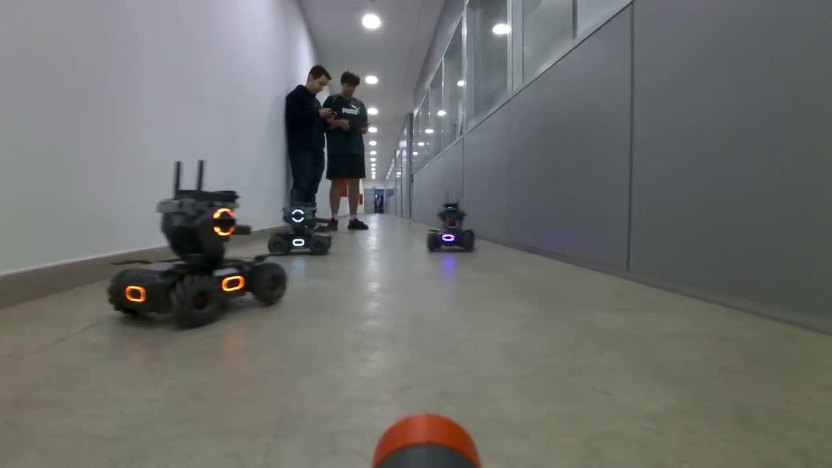
\includegraphics[width=\linewidth]{00_original.jpg}\\[-1pt]{\footnotesize Original}\end{minipage}\hfill
\begin{minipage}{0.32\textwidth}\centering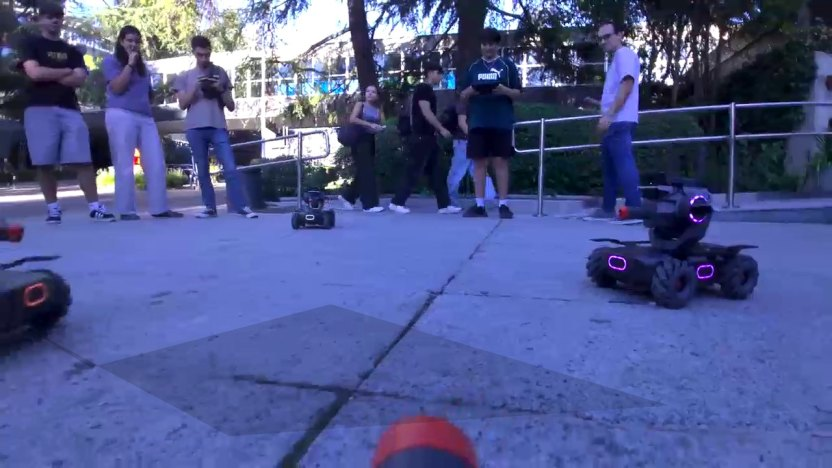
\includegraphics[width=\linewidth]{13_sombra.jpg}\\[-1pt]{\footnotesize Sombra (exterior, se usó)}\end{minipage}\hfill
\begin{minipage}{0.32\textwidth}\centering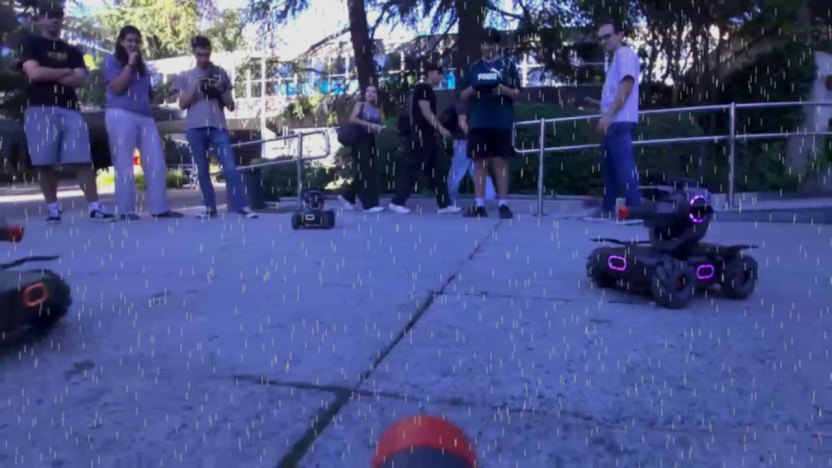
\includegraphics[width=\linewidth]{14_lluvia.jpg}\\[-1pt]{\footnotesize Llovizna (exterior, se usó)}\end{minipage}\\[4pt]
\begin{minipage}{0.32\textwidth}\centering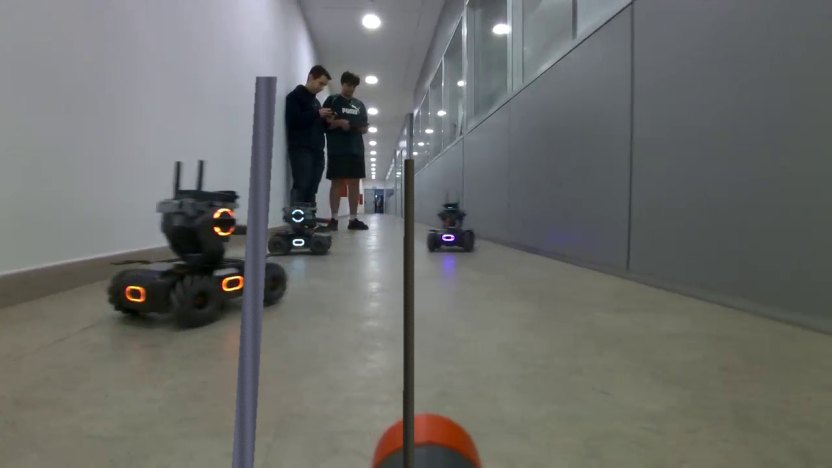
\includegraphics[width=\linewidth]{15_postes.jpg}\\[-1pt]{\footnotesize Postes con textura (se usó)}\end{minipage}\hfill
\begin{minipage}{0.32\textwidth}\centering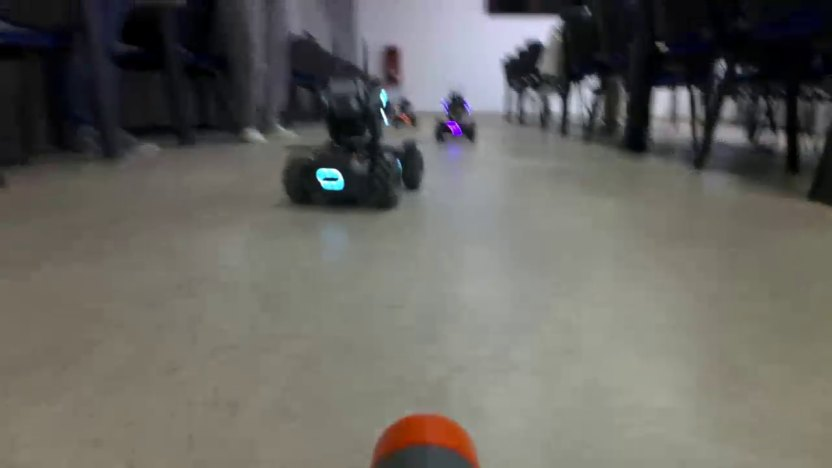
\includegraphics[width=\linewidth]{17_dif_movido.jpg}\\[-1pt]{\footnotesize Copia \emph{difficult} movida (se usó)}\end{minipage}\hfill
\begin{minipage}{0.32\textwidth}\centering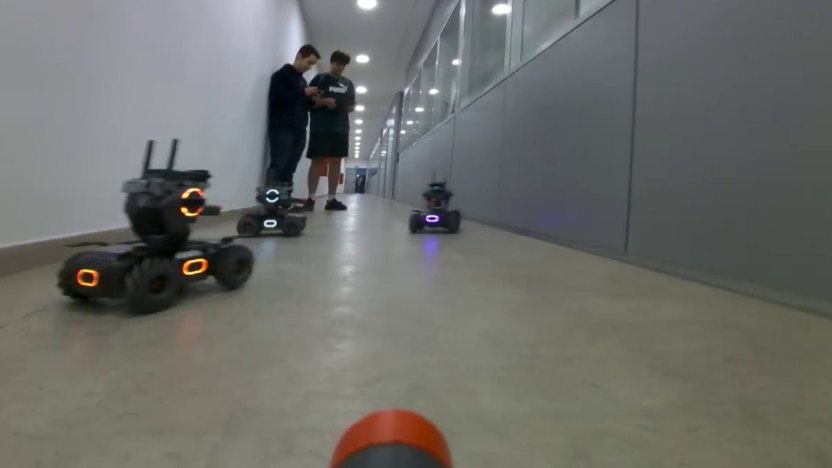
\includegraphics[width=\linewidth]{21_perspectiva.jpg}\\[-1pt]{\footnotesize Perspectiva (no se usó)}\end{minipage}
\caption{Salida real del código del aumento, con las cajas transformadas (\cod{herramientas/\allowbreak{}figuras\_\allowbreak{}aumento.py}; las 25 están en \cod{docs/\allowbreak{}informes/\allowbreak{}figuras/\allowbreak{}aumento/}).}
\end{figure}

\textbf{Datos defendibles:}
\begin{itemize}
  \item Nuestro aumento pierde el 0,7\,\% de los robots y conserva la forma (aspecto 1,10); el del notebook original, simulado, perdería el 14,1\,\% y los deformaría (1,18).
  \item Con Faster R-CNN v1, el aumento sube el AP@0,5 en validación de 0,923 a 0,942 y en \emph{difficult} de 0,552 a 0,634 (+8 pp), con un 28\,\% menos de robots perdidos (FN 115 $\rightarrow$ 83). Parte de la mejora puede deberse a que cuadruplica las imágenes y las actualizaciones.
  \item Los extras de \cod{robusto\_\allowbreak{}v1} dan lo mismo que el aumento base: 0,9426 frente a 0,9433 (en \emph{difficult}, 0,6471 frente a 0,6462). Una explicación posible es que el base ya cubría esa variabilidad; no se ha comprobado.
\end{itemize}

\begin{pregunta}{¿Se usaron para entrenar las sombras y la lluvia? ¿Y todo lo de la tabla?}
Sí. Todas las transformaciones de la tabla de la diapositiva 9 forman el perfil \cod{robusto\_\allowbreak{}v1}, con el que se entrenaron los 13 modelos de la comparación, incluido el final (\cod{faster\_\allowbreak{}rcnn\_\allowbreak{}v2\_\allowbreak{}aug\_\allowbreak{}robusto\_\allowbreak{}v1\_\allowbreak{}lr001}). Las que aparecen con «no se usó» se probaron y se descartaron con el motivo que se ve en pantalla.
\end{pregunta}

\begin{pregunta}{Si los extras no mejoran, ¿por qué se mantienen?}
Porque no empeoran (0,9426 frente a 0,9433 está dentro del ruido de una sola semilla) y cubren casos que no grabamos: exterior con sombras o llovizna, obstáculos con textura. Además validación y test son casi todo interior, así que no pueden medir bien lo que aportan en exterior.
\end{pregunta}

\begin{pregunta}{¿Por qué no CoarseDropout para las oclusiones?}
Borrar rectángulos al azar puede tapar un robot entero y dejar su caja sobre el fondo: le enseñaría a la red a detectar fondo. Los postes nunca tapan más del 25\,\% de un robot, de modo que su caja sigue siendo válida.
\end{pregunta}

\newpage
% =====================================================================
\section{Bloque 2: el modelo}\label{sec:bloque2}

\subsection{El sistema de entrenamiento}
Código en \cod{train.ipynb} y \cod{test.ipynb} (JupyterHub del laboratorio, GPU RTX 3060 de 12 GB, PyTorch 2.4.1 y torchvision 0.19.1, semilla 0). El esquema de la memoria es: datos $\rightarrow$ carga en lotes $\rightarrow$ detector $\rightarrow$ función de pérdida (RPN + clase + posición) $\rightarrow$ optimizador SGD $\rightarrow$ evaluación en validación cada época $\rightarrow$ selección del mejor \emph{checkpoint} y del umbral $\rightarrow$ test (una vez).

\begin{figure}[H]
\centering
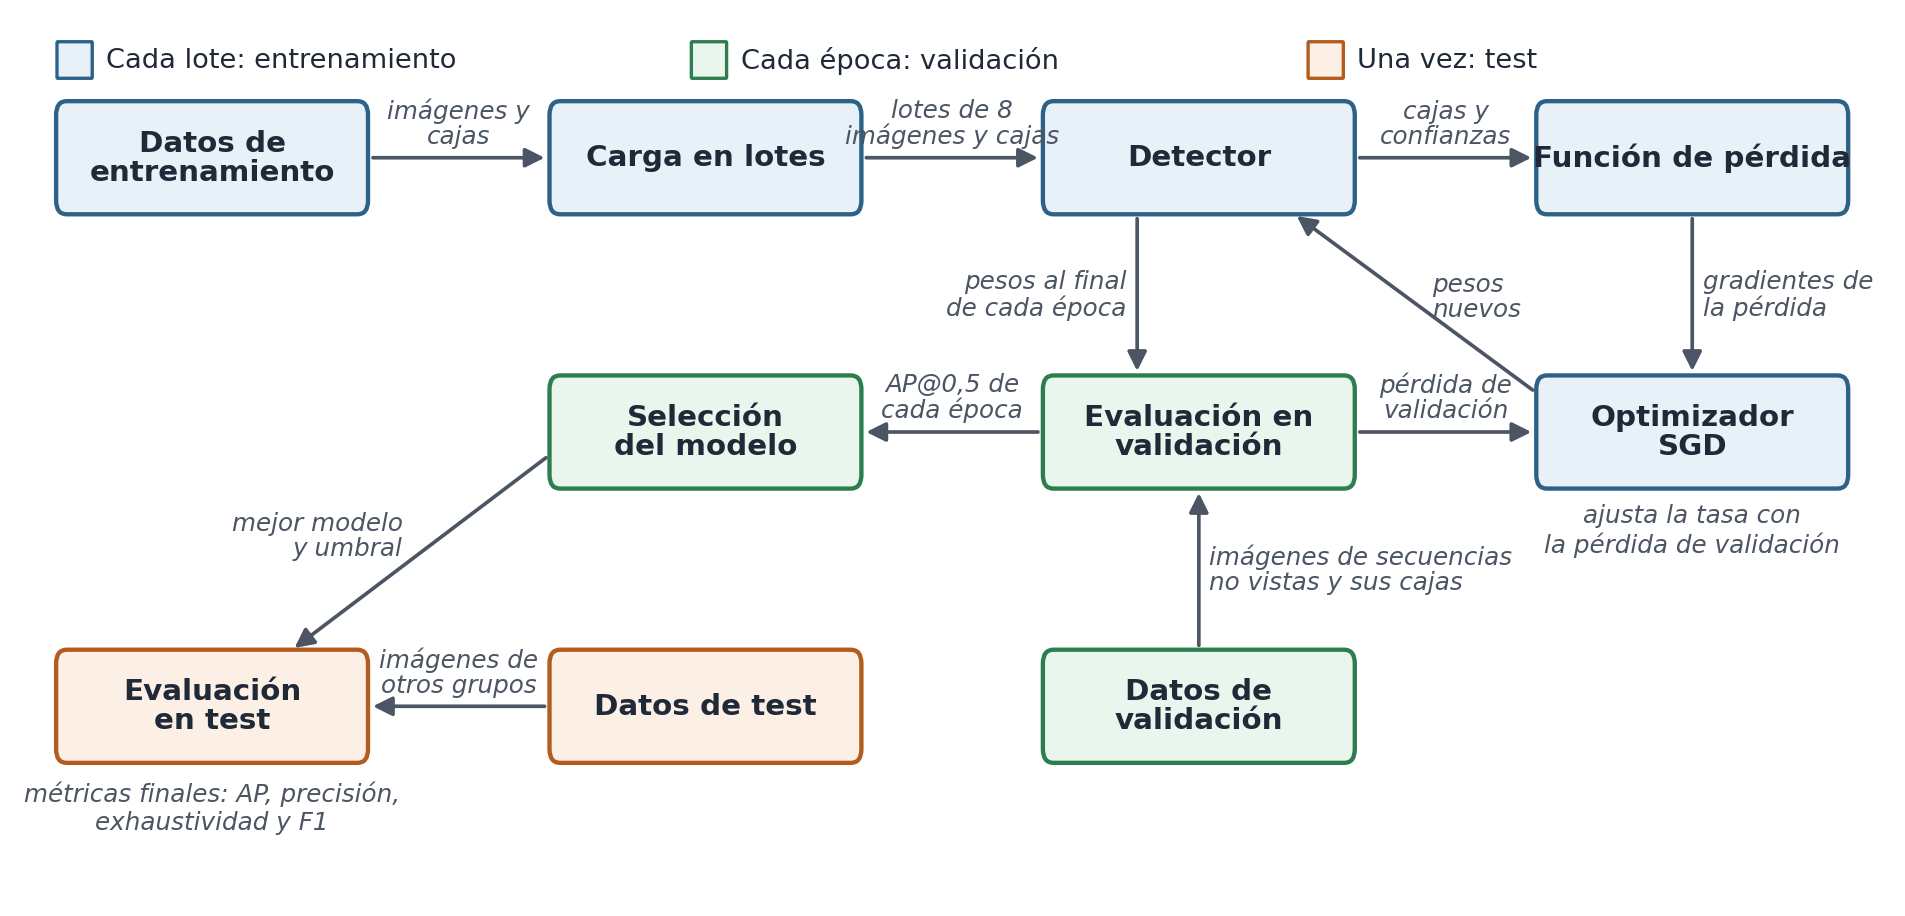
\includegraphics[width=0.9\textwidth]{sistema_entrenamiento.png}
\caption{Esquema de bloques del entrenamiento y la evaluación.}
\end{figure}

\subsection{Las siete arquitecturas}
Todas con \textbf{transfer learning} desde COCO, sustituyendo la cabeza de clasificación por una de dos clases (fondo/robot). Con 796 imágenes originales de diez vídeos sería inviable entrenar desde cero redes de decenas de millones de parámetros.

\begin{center}
\small
\begin{tabular}{@{}P{3.6cm}P{4.6cm}P{3.2cm}P{3.6cm}@{}}
\toprule
\textbf{Modelo} & \textbf{Tipo} & \textbf{Backbone} & \textbf{Para qué sirve} \\
\midrule
Faster R-CNN v1 / v2 & Dos etapas (RPN + clasificación por región) & ResNet-50 + FPN & v2 tiene mejoras de cabezas y entrenamiento \\
Faster R-CNN MobileNet & Dos etapas, ligera & MobileNetV3-L + FPN & Opción rápida (16 ms) \\
RetinaNet v1 / v2 & Una etapa, pérdida focal & ResNet-50 + FPN & Compensa el desequilibrio de anclas de fondo \\
SSD300 & Una etapa, entrada 300$\times$300 & VGG16 & Rápida, pierde robots lejanos \\
SSDlite320 & Una etapa, ligera & MobileNetV3-L & La peor (AP 0,64 en test) \\
\bottomrule
\end{tabular}
\end{center}

\textbf{Detalles que suelen preguntar:}
\begin{itemize}
  \item \textbf{FPN:} el backbone da mapas cada vez más pequeños (los primeros con detalle espacial, los últimos con información de qué hay). La FPN los recorre de arriba abajo: amplía cada mapa profundo al tamaño del anterior y lo suma tras una convolución 1$\times$1. Resultado: pirámide de mapas con información semántica en todos los niveles; los robots lejanos se buscan en los mapas grandes y los cercanos en los pequeños.
  \item \textbf{Una etapa frente a dos:} dos etapas localizan mejor (la segunda trabaja con unas mil regiones ya filtradas); una etapa es más simple y en general más rápida, pero debe separar pocos objetos de decenas de miles de anclas de fondo (lo que compensa la pérdida focal). \textbf{En nuestras medidas, con el mismo backbone la diferencia de tiempo es pequeña} (RetinaNet v1 72 ms, Faster R-CNN v1 75 ms): pesa más el tamaño del backbone y de la imagen.
  \item \textbf{Reescalado:} Faster R-CNN y RetinaNet reescalan sin deformar con dos límites (lado corto 800, salvo que el largo pase de 1333). Una imagen de 1280$\times$720 entra a 1333$\times$750, apenas un 4\,\% más grande. SSD reduce a 300$\times$300 / 320$\times$320, por eso los robots lejanos quedan minúsculos y los \emph{difficult} caen (AP 0,43 y 0,27).
\end{itemize}

\subsection{Hiperparámetros y su porqué}
\begin{itemize}
  \item \textbf{Lote 8.} Es el mayor que cabe en 12 GB (16 y 32 dan \emph{CUDA out of memory}). Pruebas cortas de tres épocas sin aumento: con 1 y 2 el AP@0,5 sube antes (más pasos por época) pero baja en la tercera; con 8 sube más regular, y los tres acaban a menos de 0,4 pp. Da unos 400 pasos por época con las 3184 imágenes. Faster R-CNN v2 y el experimento a 1024 px no caben con 8: se usan \textbf{microlotes de 4 acumulando dos gradientes} (lote efectivo 8). Se prueban 8, 4 y 2 (los que dividen a 8) y no 6, para que todos los pasos tengan 8 imágenes y sean comparables.
  \item \textbf{Por qué el lote importa:} el gradiente de un lote es una estimación del verdadero y su dispersión baja con la raíz del tamaño del lote. Ruido moderado regulariza y ayuda a salir de mínimos estrechos; demasiado obliga a bajar la tasa.
  \item \textbf{SGD, momentum 0,9, weight decay $5\cdot10^{-4}$:} el momentum promedia la dirección de unos 10 lotes ($1/(1-0{,}9)$); el weight decay penaliza los pesos grandes. Son los valores del artículo de Faster R-CNN y del tutorial de torchvision; no se tocaron porque solo se ajustó la tasa, el hiperparámetro al que el entrenamiento es más sensible. No se probaron otros optimizadores, así que no se puede decir que SGD sea mejor.
  \item \textbf{Tasa de aprendizaje.} $10^{-5}$: AP@0,5 de 0,026 tras tres épocas (casi no aprende). $10^{-4}$: mejor época 29. $10^{-3}$: mejor época 5. $2\cdot10^{-3}$: el máximo llega en la época 1--2 y luego baja más de 1 pp. $10^{-1}$: NaN desde la primera época. Entre $10^{-4}$ y $10^{-2}$ la tasa cambia sobre todo la velocidad, no el resultado.
  \item \textbf{Programador:} multiplica la tasa por 0,1 tras 5 épocas sin mejorar la pérdida de validación (mínimo $10^{-10}$). La paciencia de 5 resultó larga: el mejor \emph{checkpoint} llega entre las épocas 3 y 7 y la primera bajada en la 11. Estrategia mejor: prueba de rango de la tasa, búsqueda logarítmica alrededor y paciencia de 2--3 épocas.
  \item \textbf{Épocas:} 30 al inicio, 12 después (15 con $5\cdot10^{-4}$). En 6 de 7 modelos el mejor \emph{checkpoint} está entre las épocas 3 y 7: hay \textbf{sobreajuste temprano}, no falta de épocas. Comprobado con SSD300 a 40 épocas: el AP en validación no se mueve y la pérdida de validación sube desde la época 8.
\end{itemize}

\subsection{Métricas: definiciones exactas}
\begin{itemize}
  \item \textbf{Emparejamiento:} una detección es TP si tiene IoU $\ge$ 0,5 con un robot anotado (se emparejan por confianza, cada robot una vez); FP si no tiene pareja; un robot sin detectar es FN.
  \item \textbf{Precisión} TP/(TP+FP), \textbf{exhaustividad} (\emph{recall}) TP/(TP+FN), \textbf{F1} su media armónica.
  \item \textbf{AP:} área bajo la curva precisión--exhaustividad al variar el umbral de confianza. \textbf{AP@0,5} con IoU 0,5; \textbf{AP@0,75} exige cajas más ajustadas; \textbf{AP 0,50:0,95} promedia diez umbrales de IoU (la «mAP» de COCO; con una sola clase, mAP = AP).
  \item \textbf{AP por tamaño (COCO):} pequeños $<32^2$ px$^2$, medianos de $32^2$ a $96^2$, grandes $>96^2$. \textbf{AR@100}: exhaustividad media entre IoU 0,50 y 0,95 con hasta 100 detecciones por imagen.
  \item \textbf{Exactitud:} en detección no hay verdaderos negativos (el fondo no es un objeto y el test no tiene imágenes vacías), así que TN = 0 y la exactitud se reduce a TP/(TP+FP+FN): 0,8848 en el modelo final.
  \item Diferencias en \textbf{puntos porcentuales} (pp): de 0,9433 a 0,9465 hay 0,32 pp.
\end{itemize}

\subsection{Cronología de los experimentos}
\begin{enumerate}
  \item \textbf{Ajuste con un solo modelo} (Faster R-CNN v1, el de partida del enunciado), para no multiplicar el coste:
  \begin{center}
  \small
  \begin{tabular}{@{}lrrr@{}}
  \toprule
  \textbf{Experimento} & \textbf{Mejor época} & \textbf{AP@0,5} & \textbf{AP 0,50:0,95} \\
  \midrule
  Sin aumento, tasa $10^{-4}$ & 20 & 0,9228 & 0,5809 \\
  Con aumento, tasa $10^{-4}$ & 29 & 0,9416 & 0,6081 \\
  Con aumento, tasa $10^{-3}$ & 5 & 0,9433 & 0,6302 \\
  Con aumento, $10^{-3}$, imagen grande (1024) & 2 & 0,9465 & 0,6047 \\
  \bottomrule
  \end{tabular}
  \end{center}
  \item \textbf{Resolución 1024} (1820$\times$1024, 86\,\% más píxeles): +0,32 pp de AP@0,5 y AP pequeños 0,12 $\rightarrow$ 0,19, pero +134 FP (190 $\rightarrow$ 324), AP@0,75 $-$4,7 pp, F1 $-$3,15 pp y +62\,\% de latencia (75 $\rightarrow$ 122 ms). \textbf{Se descarta}; además la imagen normal gana en 7 de las 11 secuencias de validación.
  \item \textbf{Cadena de 13 entrenamientos} (siete arquitecturas + tres tasas para las tres mejores) con el perfil \cod{robusto\_\allowbreak{}v1}, automatizada con \cod{herramientas/\allowbreak{}cadena\_\allowbreak{}entrenamientos.py} (comprobaciones previas, reanudable, microlotes automáticos). 21,8 horas de GPU.
  \item \textbf{Tasa en los tres mejores} ($5\cdot10^{-4}$, $10^{-3}$, $2\cdot10^{-3}$): diferencias de menos de 0,22 pp. Se mantiene $10^{-3}$ porque iguala a $5\cdot10^{-4}$ en menos épocas.
  \item \textbf{Test, una sola vez por modelo}, con el umbral fijado antes en validación (mejor F1).
\end{enumerate}

\textbf{La regla de selección se escribió antes de abrir el test} (\cod{docs/\allowbreak{}seleccion\_\allowbreak{}modelo\_\allowbreak{}final.md}, 24/10): mayor AP@0,5 en validación; si la diferencia es $<$0,5 pp (una sola semilla) se considera empate y se prefiere el más barato; el test no se usa para elegir nada.

\subsection{Resultados en test}
\begin{center}
\small
\begin{tabular}{@{}lrrrrrrr@{}}
\toprule
\textbf{Modelo} & \textbf{AP val.} & \textbf{AP test} & \textbf{Diff.\ test} & \textbf{Umbral} & \textbf{F1} & \textbf{FP/FN} & \textbf{ms} \\
\midrule
\textbf{Faster R-CNN v2} & 0,9513 & \textbf{0,9523} & \textbf{0,6921} & 0,95 & 0,9389 & 94/115 & 99,5 \\
RetinaNet v2 & 0,9447 & 0,9457 & 0,6313 & 0,65 & 0,9233 & 98/161 & 67 \\
Faster R-CNN v1 & 0,9426 & 0,9355 & 0,6057 & 0,90 & 0,9237 & 134/129 & 75 \\
RetinaNet v1 & 0,9396 & 0,9362 & 0,6273 & 0,65 & 0,9218 & 133/136 & 72 \\
Faster R-CNN MobileNet & 0,9281 & 0,9240 & 0,5744 & 0,55 & 0,9142 & 147/148 & 16 \\
SSD300 & 0,9008 & 0,8797 & 0,4316 & 0,25 & 0,8648 & 135/307 & 12,5 \\
SSDlite320 & 0,6823 & 0,6412 & 0,2742 & 0,20 & 0,6571 & 384/691 & 4 \\
\bottomrule
\end{tabular}
\end{center}

\begin{itemize}
  \item \textbf{Test confirma validación:} en el modelo final el AP es prácticamente el mismo (0,9513 $\rightarrow$ 0,9523). Los ResNet-50 apenas cambian; las SSD pierden más.
  \item \textbf{Modelo final:} Faster R-CNN v2, lr $10^{-3}$, época 3, umbral 0,95. Con él: 1606 TP, 94 FP, 115 FN; precisión 0,9447, exhaustividad 0,9332 (0,9717 en normales y 0,7259 en \emph{difficult}). AP@0,75 = 0,6005 y AP 0,50:0,95 = 0,5724: \emph{encuentra casi todos, pero muchas cajas no se ajustan tanto}.
  \item \textbf{Dónde falla:} 74 de los 115 FN (64\,\%) son \emph{difficult}, que son solo el 16\,\% de los robots.
  \item \textbf{Alternativa rápida:} Faster R-CNN MobileNet, 6 veces más rápido (16 ms), AP 0,924.
  \item \textbf{Mejor en casi todo:} v2 gana en AP@0,5, AP, precisión, exhaustividad, F1, exactitud y en todas las métricas de los \emph{difficult}; v1 lo supera en AP@0,75 y las RetinaNet en AR@100.
\end{itemize}

\textbf{El compromiso del umbral} (modelo final en test):
\begin{center}
\small
\begin{tabular}{@{}rrrrrrr@{}}
\toprule
\textbf{Umbral} & \textbf{TP} & \textbf{FP} & \textbf{FN} & \textbf{Precisión} & \textbf{Exhaust.} & \textbf{Exh. \emph{difficult}} \\
\midrule
0,05 & 1678 & 1011 & 43 & 0,624 & 0,975 & 0,900 \\
0,50 & 1653 & 226 & 68 & 0,880 & 0,961 & 0,841 \\
0,90 & 1627 & 109 & 94 & 0,937 & 0,945 & 0,770 \\
\textbf{0,95} & \textbf{1606} & \textbf{94} & \textbf{115} & \textbf{0,945} & \textbf{0,933} & \textbf{0,726} \\
\bottomrule
\end{tabular}
\end{center}

\begin{figure}[H]
\centering
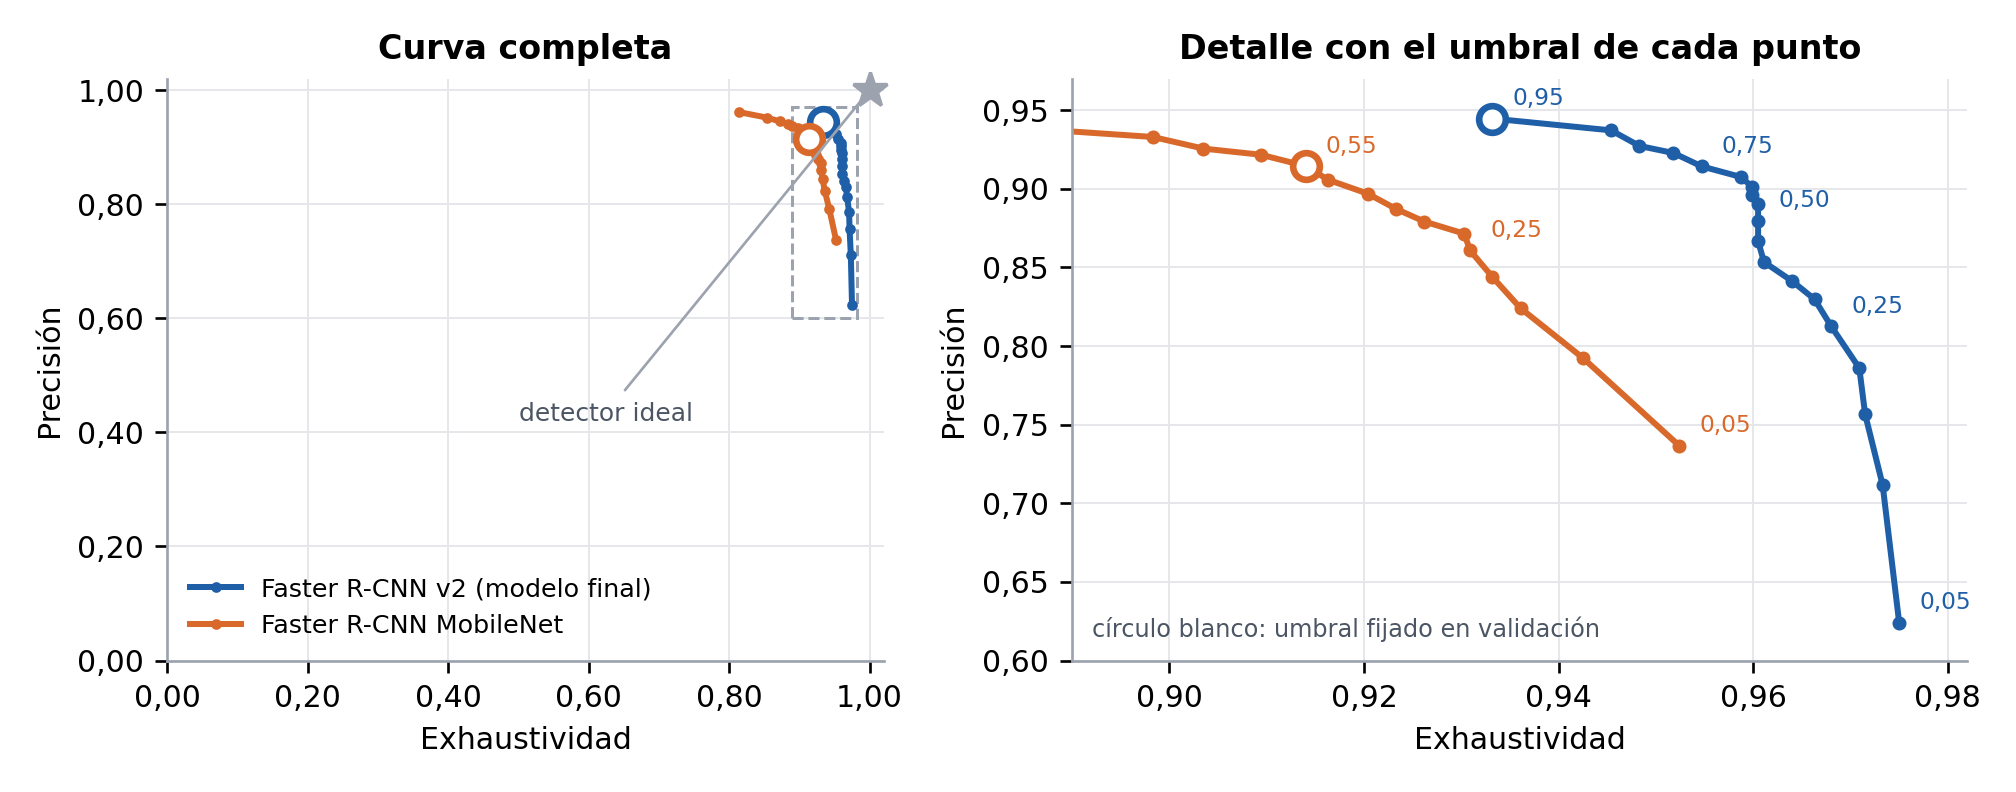
\includegraphics[width=\textwidth]{curva_pr.png}
\caption{Curva precisión--exhaustividad en test del modelo final y de Faster R-CNN MobileNet.}
\end{figure}

\subsection{Los 94 falsos positivos, uno a uno}
Se revisaron a mano los 94 FP del modelo final en test (\cod{docs/\allowbreak{}revision\_\allowbreak{}fp\_\allowbreak{}test.csv}, repetible):

\begin{center}
\begin{tabular}{@{}P{5.4cm}rp{7.4cm}@{}}
\toprule
\textbf{Tipo} & \textbf{N.\textordmasculine} & \textbf{Detalle} \\
\midrule
Robots sin anotar en el XML & 59 & Cortados por el borde, movidos, lejanos o tapados por otro robot: los que nuestro criterio sí anotaría \\
Caja mal ajustada o repetida & 31 & 14 son la única caja de un robot anotado pero con IoU $<$ 0,5; 14 una segunda caja parcial; 3 juntan dos robots en una \\
No son robots & 4 & Tres sillas en penumbra y un coche aparcado \\
\bottomrule
\end{tabular}
\end{center}

Con los 59 robots anotados, la precisión pasaría de \textbf{0,945 a 0,979}. Las etiquetas \textbf{no se corrigieron} para conservar la comparación con otros grupos. En test, el modelo acierta todo (sin FP ni FN) en 546 de las 718 imágenes.

\begin{contar}
«De los 94 falsos positivos, solo 4 no son robots. 59 son robots que nosotros habríamos anotado y faltan en los XML de otros grupos. Lo que de verdad falla el modelo son los \emph{difficult}: 74 de los 115 robots que no encuentra.»
\end{contar}

\subsection{Limitaciones honestas (úsalas, suman puntos)}
\begin{itemize}
  \item \textbf{Una sola semilla:} diferencias $<$0,5 pp no son concluyentes (los cuatro ResNet-50 están a menos de 1,2 pp).
  \item \textbf{Etiquetas de validación/test de otros grupos}: no siguen del todo nuestro criterio. Caso confirmado en validación: \cod{PIDS2024\_\allowbreak{}GR02\_\allowbreak{}0001} con 4 robots visibles y 1 sola caja. En test, 59 de los 94 FP son robots sin anotar.
  \item \textbf{Secuencias difíciles:} en test, \cod{PIDS2025\_\allowbreak{}GR02\_\allowbreak{}0009} pierde 40 de 204 robots y \cod{PIDS2025\_\allowbreak{}GR04\_\allowbreak{}0000} pierde 10 de 21.
  \item \textbf{Robots lejanos:} en validación, AP de objetos pequeños de 0,12--0,19 (Faster R-CNN v1); no hay cajas originales de menos de 30 px.
  \item El \emph{checkpoint} y el umbral se eligieron con validación: sus cifras son algo optimistas (por eso existe el test).
  \item Parte de la mejora del aumento puede ser simplemente tener más imágenes y más actualizaciones por época.
\end{itemize}

\begin{pregunta}{¿Por qué umbral 0,95, tan alto?}
Es el de mejor F1 en \emph{validación} (0,9361), fijado antes de ver el test. En test, el mejor posible habría sido 0,9413 con umbral 0,90: solo 0,24 pp más, así que el umbral generaliza. Además, en la demo \textbf{es preferible no disparar a algo que no es un robot}: un falso positivo es peor que perder un objetivo difícil.
\end{pregunta}

\begin{pregunta}{¿Por qué el modelo final y no el MobileNet, que es 6 veces más rápido?}
Por mayor AP y mejor F1, sobre todo en \emph{difficult} (0,69 frente a 0,57). La latencia se resolvió llevando la inferencia a la GPU del portátil (unos 108 ms por imagen en la demo), que basta para disparar en marcha. MobileNet queda como plan B.
\end{pregunta}

\begin{pregunta}{¿Por qué la época 3? ¿No es muy pronto?}
Porque Faster R-CNN v2 sobreajusta pronto: a partir de ahí la pérdida de entrenamiento sigue bajando pero la de validación sube. Se guarda el \emph{checkpoint} con mayor AP@0,5 en validación, no el último. Con 3184 imágenes y lote 8, tres épocas son unos 1200 pasos, y el modelo parte de COCO.
\end{pregunta}

\begin{pregunta}{En test el AP de pequeños es 0,47, ¿no decíais 0,12--0,19?}
Son medidas distintas: 0,12--0,19 es Faster R-CNN v1 en \emph{validación} (800 frente a 1024 px), donde el 2,5\,\% de las cajas mide menos de 30 px. En test, con v2, es 0,47, pero test casi no tiene robots pequeños (0,5\,\% de menos de 30 px), así que esa cifra sale de muy pocas cajas.
\end{pregunta}

\newpage
% =====================================================================
\section{Bloque 3: el robot}\label{sec:bloque3}

\subsection{Arquitectura del software}
Todo en \cod{ENTREGA 2/\allowbreak{}WEEK3}. La separación de responsabilidades es la clave para explicarlo:

\begin{center}
\begin{tabular}{@{}lp{10.5cm}@{}}
\toprule
\cod{circuito.py} & Dice \textbf{qué} hacer: modelo, umbral, paradas, rivales, velocidades. Es lo único que se ajusta en el laboratorio. \\
\cod{recorrido.py} & Convierte el plano (metros) en movimientos del chasis. \\
\cod{demo.py} & Decide \textbf{cuándo} hacer cada cosa (el director: barrido, puntería, ataque en marcha, baile). \\
\cod{demo\_\allowbreak{}utils.py} & Sabe \textbf{cómo} se hace cada acción con el robot: cámara, detector, puntería, avance recto, LED, sonido. \\
\cod{demo\_\allowbreak{}gpu.py} & La misma demo, cambiando el detector por uno en GPU (proceso aparte). \\
\cod{simulacion.py} & Robot simulado: la demo completa se prueba sin RoboMaster, con imágenes de test. \\
\cod{rival/\allowbreak{}} & Kit para mover el rival 2 desde otro portátil. \\
\cod{mando/\allowbreak{}} & Interfaz web de control manual. \\
\bottomrule
\end{tabular}
\end{center}

\textbf{Restricción de partida:} el SDK del RoboMaster solo funciona con \textbf{Python 3.8}, y el PyTorch de 3.8 no admite la RTX 5070 del portátil. En CPU cada imagen tarda unos 2,3 s. \emph{Esa latencia condiciona todo el bloque}: el robot tiene que repartir el tiempo entre girar, mirar y disparar.

\textbf{Solución:} un proceso aparte con Python 3.11 y PyTorch con CUDA 12.8 carga el mismo modelo; la demo le manda cada imagen en JPEG por HTTP local (\cod{127.0.0.1:8767}). En la demo oficial, \textbf{unos 108 ms por imagen}, con las mismas detecciones. Si la GPU falla, esa imagen va a CPU; tras 3 fallos seguidos, el resto de la demo en CPU. Funciona con la RTX 5070 del portátil y con la RTX 3060 del laboratorio.

\begin{clave}
Es una buena respuesta a «¿qué problema técnico fue el más gordo?»: no fue la red, fue integrar un SDK atado a Python 3.8 con una GPU moderna. Y la solución fue arquitectónica (proceso separado + respaldo), no un parche.
\end{clave}

\subsection{El circuito}
Plano en metros con origen en la salida; $x$ adelante, $y$ a la derecha. Las ruedas \textbf{mecanum} permiten moverse de lado y hacia atrás sin girar el chasis. Todos los tramos se midieron en el laboratorio. La demo dura unos 2 min 18 s.

\begin{figure}[H]
\centering
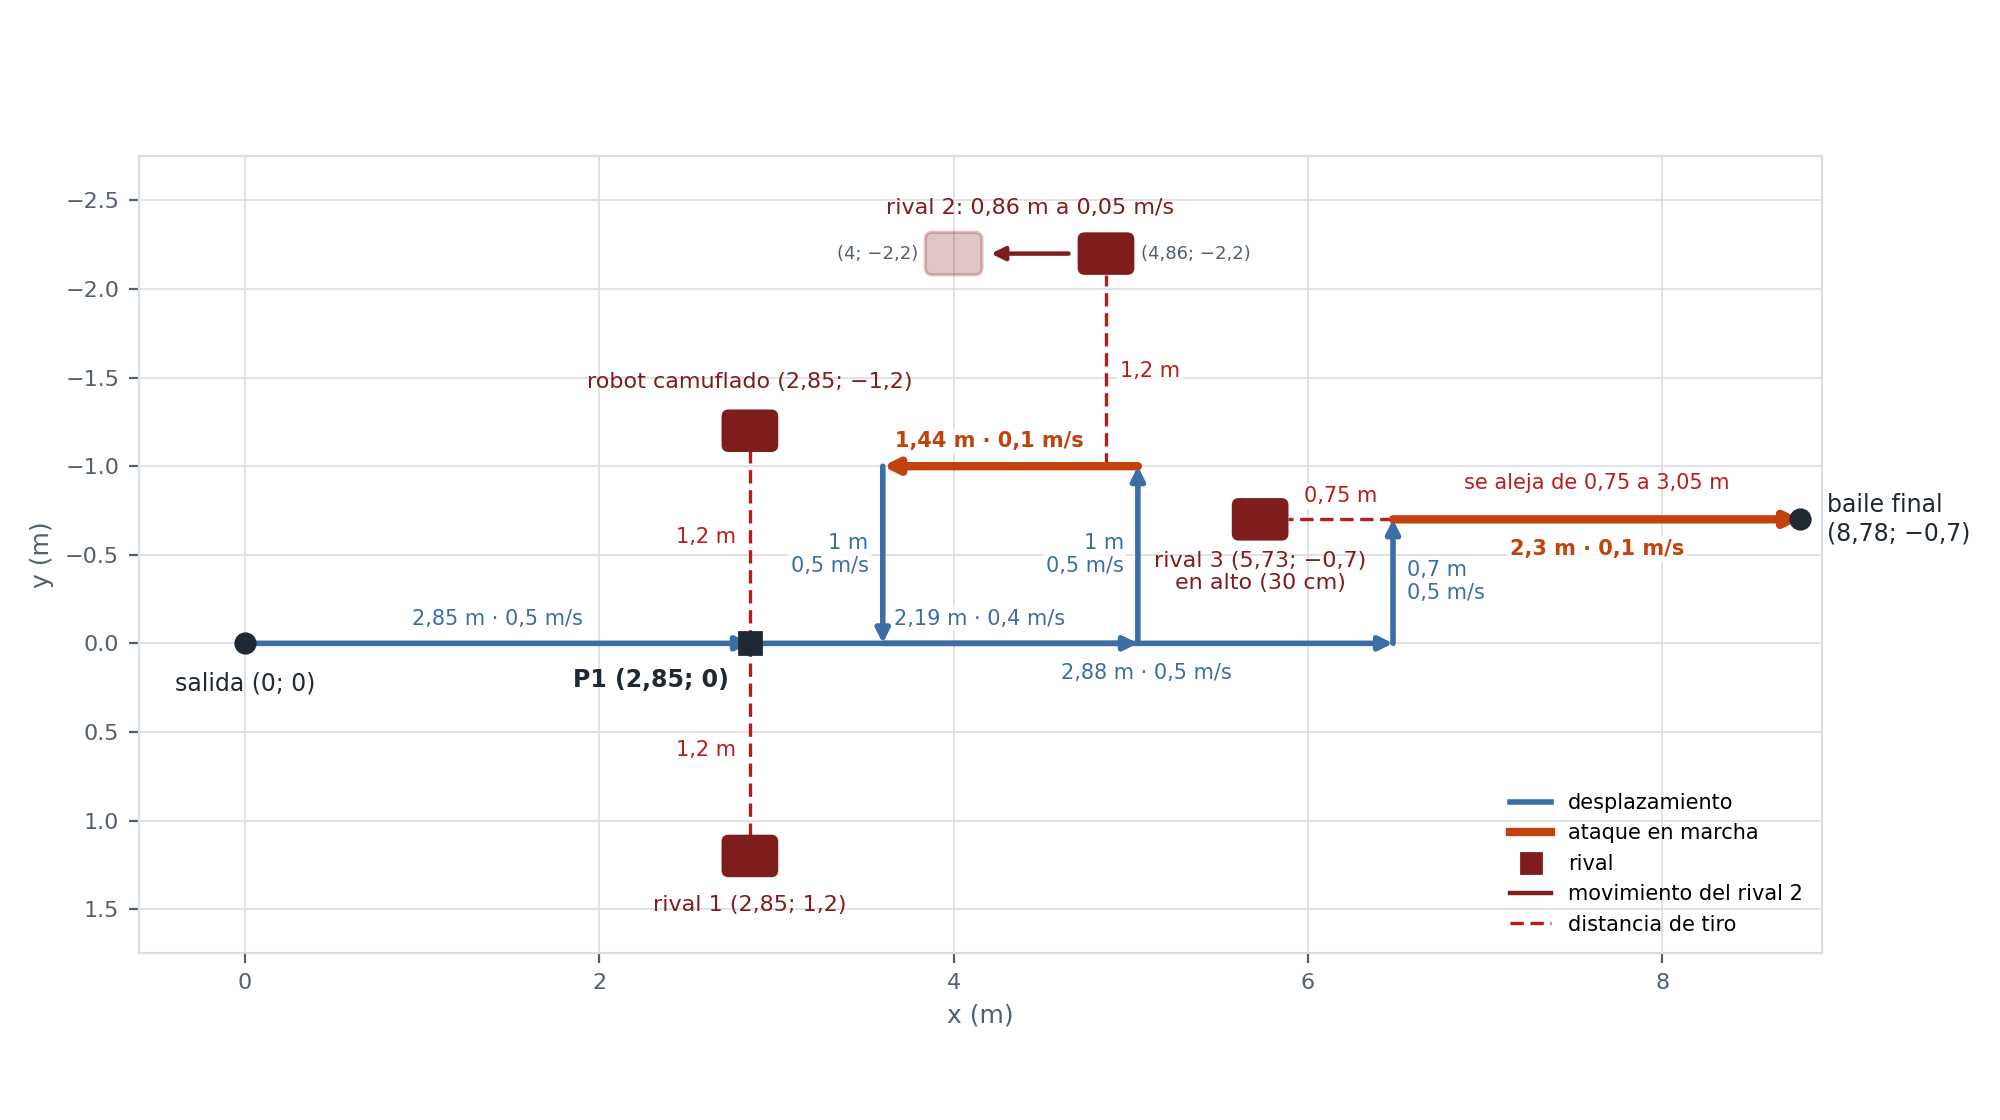
\includegraphics[width=0.88\textwidth]{circuito_demo.png}
\caption{Recorrido de la demo (azul: desplazamientos; naranja: ataques en marcha; granate: rivales).}
\end{figure}

\begin{center}
\small
\begin{tabular}{@{}P{1.3cm}P{3.4cm}P{1.9cm}P{1.7cm}P{5.6cm}@{}}
\toprule
\textbf{Tramo} & \textbf{Movimiento} & \textbf{Velocidad} & \textbf{Tiempo} & \textbf{Acción} \\
\midrule
P1 & 2,85 m adelante & 0,5 m/s & $\approx$6 s & Suena un Fórmula 1 ajustado a la recta (6,4 s) \\
P1 & Parada & -- & -- & Torreta a 90\gr: rival 1; a $-90$\gr: robot camuflado \\
R1 & 2,19 m adelante & 0,4 m/s & $\approx$6 s & -- \\
R1 & 1 m a la izquierda & 0,5 m/s & $\approx$2,5 s & -- \\
R1 & 1,44 m \textbf{atrás} & 0,1 m/s & $\approx$14,5 s & Torreta a la izquierda: \textbf{rival 2, que se mueve} 0,86 m en paralelo a 0,05 m/s \\
R1 & 1 m a la derecha & 0,5 m/s & $\approx$2,5 s & -- \\
R2 & 2,88 m adelante & 0,5 m/s & $\approx$6 s & -- \\
R2 & 0,7 m a la izquierda & 0,5 m/s & $\approx$2 s & -- \\
R2 & 2,3 m adelante & 0,1 m/s & $\approx$23 s & Torreta a 180\gr: \textbf{rival 3, escondido} \\
Final & Baile & -- & -- & Super Estrella, torreta, chasis y LED \\
\bottomrule
\end{tabular}
\end{center}

\textbf{Por qué se retrocede a 0,1 m/s en los ataques en marcha:} el tiempo se reparte así: girar la torreta 90\gr{} (3 s) + encontrar y fijar al rival + aviso de voz (1,4 s) + ráfaga (6,2 s). A 0,1 m/s los 1,44 m duran $\approx$14,5 s, suficiente para todo. La velocidad sale de \emph{sumar tiempos}, no de ajustar a ojo.

\textbf{Ataque en marcha = tres tareas a la vez:} el chasis mantiene su velocidad (sus órdenes caducan a los 0,5 s y su tarea las renueva sin pausa), la torreta busca y sigue al rival, y una tercera lanza el aviso y la ráfaga. Así el chasis no espera a la torreta ni a la ráfaga.

\subsection{Detección, puntería y disparo: lo que hay que entender}
\begin{enumerate}
  \item \textbf{Píxeles a grados} (\cod{auto\_\allowbreak{}aim}): $\alpha = \arctan(\text{desvío}/f)$ con $f = \text{ancho}/(2\tan 60^\circ)$, escalado por 90/120 porque el campo de visión medido es $\approx$90\gr{} y no 120\gr. Es la función que da la plantilla de la asignatura y la hemos extendido a vertical (\cod{auto\_\allowbreak{}pitch}).
  \item \textbf{Distancia} sin sensor: $d = \text{ALTURA\_ROBOT} / (2\tan(\text{alto angular}/2))$, con \cod{ALTURA\_\allowbreak{}ROBOT} = 0,35 m. Aproximada, pero separa 1,3 m de 2,6 m; sirve para descartar robots del fondo.
  \item \textbf{Puntería por pasos:} se gira hacia el ángulo estimado, se toma otra imagen, se mide el error y se corrige hasta 4 veces; se dispara cuando el error es $<$3\gr{} o $<$30\,\% del ancho de la caja. Si al confirmar no ve nada, \textbf{no dispara}.
  \item \textbf{Ráfaga:} 20 disparos, uno cada 0,3 s (el enunciado pide 12; los 8 de más cubren impactos no registrados). Cada disparo se lanza en su instante exacto respecto al audio de 6,2 s.
  \item \textbf{Giros grandes en tramos de 45\gr} porque el SDK solo garantiza unos 55\gr{} por orden.
  \item \textbf{Seguimiento en marcha:} durante la ráfaga la torreta sigue al rival con su velocidad angular estimada más una corrección limitada al 80\,\% del error. De lo que llega en los últimos 0,2 s se analiza la imagen más nítida (varianza del laplaciano). Una detección a más de \cod{SALTO\_\allowbreak{}MAX} = 25\gr{} de donde se espera al robot fijado se trata como \emph{otro} robot.
  \item \textbf{LED:} ámbar buscando, rojo parpadeando al disparar, verde tras eliminar a un rival.
\end{enumerate}

\subsection{Decisiones del circuito y lo que ceden (diapositiva 21)}
\begin{longtable}{@{}P{3.6cm}P{5.5cm}P{5.4cm}@{}}
\toprule
\textbf{Decisión} & \textbf{Qué gana} & \textbf{Qué cede} \\
\midrule
\endhead
Ninguna caja más alta que media imagen es un robot (\cod{ALTO\_\allowbreak{}MAX\_\allowbreak{}ROBOT}) & Un robot así estaría a $<$0,5 m. El 11/11 las sillas azules cercanas daban 0,95--0,99 con cajas de 650--720 px; un robot, 100--200 px & No dispararía a un robot pegado a la cámara \\
En P1, nada a más de 2 m (\cod{distancia\_\allowbreak{}max}) & Ignora robots de otros grupos al fondo (uno dio 0,98 a unos 3 m) & Depende de una distancia aproximada. \textbf{No se aplicaba en los ataques en marcha} \\
Umbral 0,95; 0,7 solo hacia el camuflado & Ningún disparo a sillas o personas & Robots tapados o borrosos no llegan \\
Error $<$3\gr{} o 30\,\% del ancho, hasta 4 correcciones & Dispara centrado & Más tiempo por objetivo \\
Ráfaga de 20 & Cubre 8 impactos no registrados & 6,2 s por objetivo \\
0,1 m/s en los ataques en marcha & Da tiempo a girar, ver, avisar y disparar & Tramos lentos \\
Siempre la imagen más reciente & Nada de imágenes viejas o dañadas & Un hilo extra leyendo el vídeo \\
\bottomrule
\end{longtable}

\subsection{Los problemas reales y cómo se resolvieron}
Esta es la parte más rica para explicar con honestidad.

\begin{longtable}{@{}P{4cm}P{5.4cm}P{5.1cm}@{}}
\toprule
\textbf{Problema} & \textbf{Causa} & \textbf{Solución} \\
\midrule
\endhead
El robot detectaba al rival (0,96--1,00) pero no disparaba; imágenes con franjas o viejas & El SDK deja el vídeo en una cola de 64 imágenes que nadie vacía mientras se analiza: se llena y llegan imágenes antiguas o dañadas & Un hilo lee el vídeo siempre y guarda solo la última; cada análisis espera una imagen tomada con la torreta ya quieta \\
La torreta apuntaba donde \emph{estaba} el robot, no donde está & La imagen llega con retraso por wifi (se estima en unos 0,25 s, \cod{RETARDO\_\allowbreak{}CAMARA}) & Se guarda un historial de ángulos de torreta y se usa el ángulo \textbf{del instante de la foto} (\cod{angulo\_\allowbreak{}en}) \\
Rival en movimiento & El robot se mueve mientras se analiza la imagen & Velocidad angular prevista por geometría + corrección limitada al 80\,\% del error; imagen más nítida de los últimos 0,2 s \\
El robot se desviaba al ir recto & Las ruedas decían «recto» pero el chasis giraba & Bucle de control con odometría + \textbf{IMU}: rampa de frenada, corrección de deriva lateral y de rumbo \\
La IMU «giraba» parada (8\gr{} en 60 s) & Deriva del sensor & Si lleva $>$3 s quieto, el cambio se toma como deriva y se mueve la referencia \\
Corrección de rumbo en el sentido equivocado & Se supuso el signo & Ahora se \textbf{mide}: giro de prueba de 0,3 s y se mira hacia dónde cambia la IMU \\
\texttt{chassis.move} iba a $\approx$0,06 m/s & El SDK no convierte a m/s reales & Se usa \texttt{drive\_speed} \\
Sillas cercanas detectadas como robot & Cajas enormes con mucha confianza & Ninguna caja más alta que media imagen es un robot \\
Sonido de la SCAR apenas audible & Clip de 0,19 s, el altavoz corta el inicio, y se subía por FTP en cada disparo & +9 dB, 0,3 s de silencio al principio y una sola pista de 6,2 s \\
Tramos del plano cortos & El plano no coincidía con el suelo real & +15\,\% en los tramos tras el túnel, medido en el laboratorio \\
\bottomrule
\end{longtable}

\subsection{El robot camuflado (y la lección sobre aliados)}
La idea inicial era un \textbf{señuelo}: algo con aspecto de robot al que \emph{no} disparar. Se probó con un RoboMaster disfrazado de detective y cuatro robots «aliados» generados con IA y marcados en verde. \textbf{Resultado: el detector los reconoce a todos como robots} (confianzas de 92,7 a 99,9\,\%; dispararía en 23 de 25 pruebas). Tapando una sola parte del detective la confianza apenas baja; solo cae al 52\,\% si se tapan chasis, ruedas y cañón a la vez. En cambio, un círculo, una caja o una caja con ruedas dibujados no dan ninguna detección. Conclusión: el modelo ha aprendido el \emph{concepto} de robot, no una pieza.

Así la idea se transformó: el disfrazado pasa a ser un objetivo más (el «robot camuflado» de P1) y la identificación de aliados queda como \textbf{trabajo futuro con una marca de color}, no una forma: los aliados tienen entre 5,7 y 12,5\,\% de verde intenso en su caja y el detective 0\,\%, así que una regla «$>$2\,\% de verde = aliado» los separa. No se implementó por riesgo de falsos positivos con la luz del laboratorio o un fondo verde. Es como en las competiciones de RoboMaster, donde los equipos se distinguen por el color de las luces.

\textbf{Impreso frente a pantalla} (webcam del portátil, mismo detector): en papel, de 0,96 a 0,99 si ocupa de un tercio a la mitad del alto, 0,87--0,92 a un cuarto y 0,53 lejos; en tableta, 0,29--0,63 (el brillo hace que la cámara baje la exposición). Por eso se imprimió en A3 mate. Con la cámara del robot desde P1 dio de 0,72 a 0,97, casi siempre por debajo de 0,95: hacia ese lado se usa un \textbf{umbral de 0,7}, solo con cajas de menos de media imagen.

\subsection{Resultados de la demo oficial (12/11, en clase)}\label{sec:demo}
Con el detector en GPU. El robot cruzó el túnel de sillas, se paró en P1 y disparó 20 veces al \textbf{rival 1} (confianza 1,00) y otras 20 al \textbf{robot camuflado} (0,99). En R1 disparó otras 20 al \textbf{rival 2} mientras los dos se movían (1,00). Una detección pequeña junto al rival 1, a unos 3 m y fuera del circuito, se descartó por la distancia. Al \textbf{rival 3} lo detectó con 1,00, pero no lo eliminó.

\begin{figure}[H]
\centering
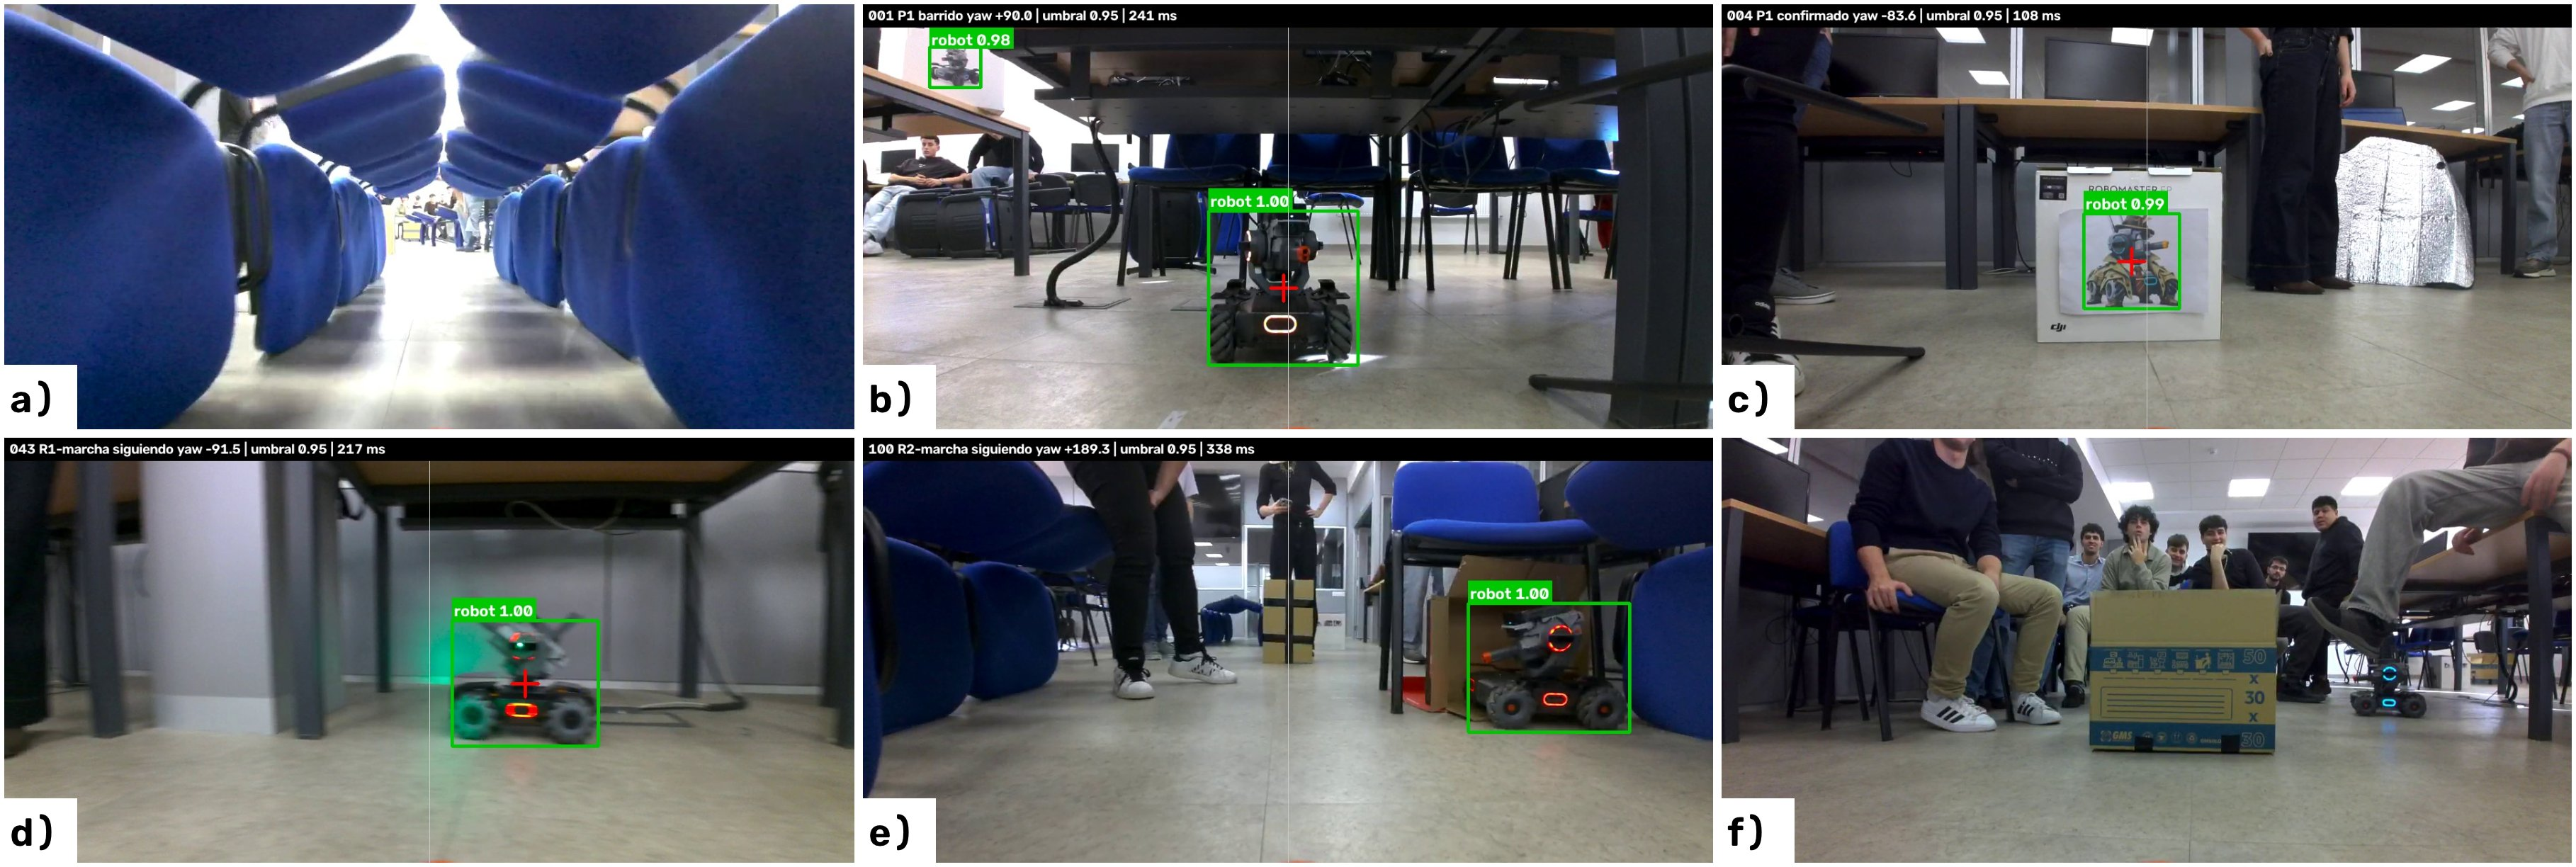
\includegraphics[width=0.95\textwidth]{demo_oficial.jpg}
\caption{Cámara del robot en la demo oficial: túnel, rival 1, camuflado, rival 2, rival 3 y baile.}
\end{figure}

\subsection{Por qué no se eliminó al rival 3}\label{sec:rival3}
La causa se comprobó en el registro de la demo (\cod{registro.csv}, imágenes 058 a 101) y en sus imágenes:

\begin{enumerate}
  \item Con la torreta a 180\gr, la primera imagen por encima del umbral mostraba \textbf{otro robot, al fondo y bajo una silla} (0,99), en el borde derecho. El rival 3 todavía no se veía.
  \item La demo fijó ese robot, sonó el aviso, giró la torreta 40\gr{} hacia él (a 220\gr) y lanzó la ráfaga.
  \item En la imagen siguiente apareció el rival 3 (1,00), pero \textbf{entre 30\gr{} y 36\gr{} a la derecha} de la línea de tiro. Como el seguimiento toma por otro robot cualquier detección a más de \cod{SALTO\_\allowbreak{}MAX} = 25\gr{} de donde espera al fijado, \textbf{lo ignoró en las 43 imágenes siguientes}.
  \item La torreta siguió girando a la velocidad prevista con el plano, unos 5\gr/s hacia atrás (de 220\gr{} a 188\gr), y los 20 disparos le pasaron por la izquierda.
  \item Lo habría evitado el \textbf{filtro de distancia de P1}, que en los ataques en marcha no se aplicaba: el robot del fondo estaba demasiado lejos.
\end{enumerate}

\begin{figure}[H]
\centering
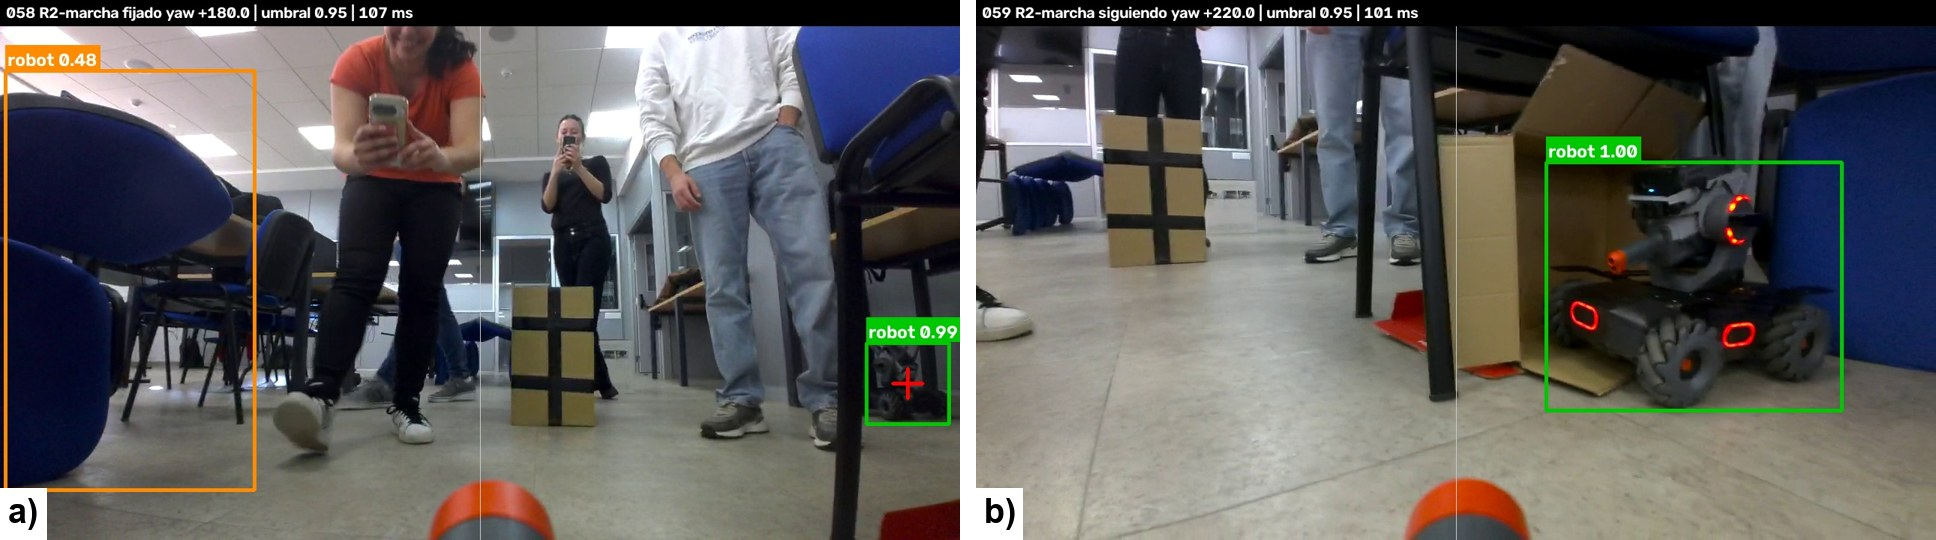
\includegraphics[width=0.95\textwidth]{7_rival3_causa.jpg}
\caption{a) Imagen 058: con la torreta a 180\gr{} la demo fija el robot del fondo (0,99). b) Imagen 059: tras girar a 220\gr, el rival 3 (1,00) queda a la derecha de la línea de tiro y se descarta.}
\end{figure}

\begin{contar}
«La detección fue buena: el rival 3 salió con 1,00. Falló a quién fijamos: el primer robot por encima del umbral era uno del fondo, y una vez fijado, la demo trató al rival 3 como otro robot por estar a más de 25\gr. El filtro de distancia que usamos en P1 lo habría descartado; no lo aplicábamos en marcha.»
\end{contar}

\begin{pregunta}{¿No era SEGUIMIENTO una mejora desactivada?}
\cod{SEGUIMIENTO} controla el seguimiento en las paradas, y está a \cod{False}. Los ataques en marcha tienen su propio seguimiento, siempre activo (si no, no se podría disparar al rival 2 mientras se mueve), y ese es el que usa \cod{SALTO\_\allowbreak{}MAX}.
\end{pregunta}

\subsection{El intento sorpresa del profesor}
Puso en P1 un robot tapado con una tela (0,85--0,91) y la foto de un robot entre humo (0,59): \textbf{no disparó a ninguno} (bajo el umbral 0,95). En la recta final puso un robot con partes rojas, de un modelo que no está en nuestros datos: lo detectó (0,96--0,99, subiendo en unos 3 s) y le disparó. Con la interfaz y desde un ángulo mejor, el robot tapado sí llegó a 0,97 y el disparo automático le disparó.

\emph{Lectura honesta:} el detector generaliza a robots distintos (parte de COCO y nuestras imágenes solo le enseñan qué es un robot), pero un robot tapado o una imagen borrosa no alcanzan 0,95; es el precio de un umbral alto para evitar falsos positivos.

\begin{figure}[H]
\centering
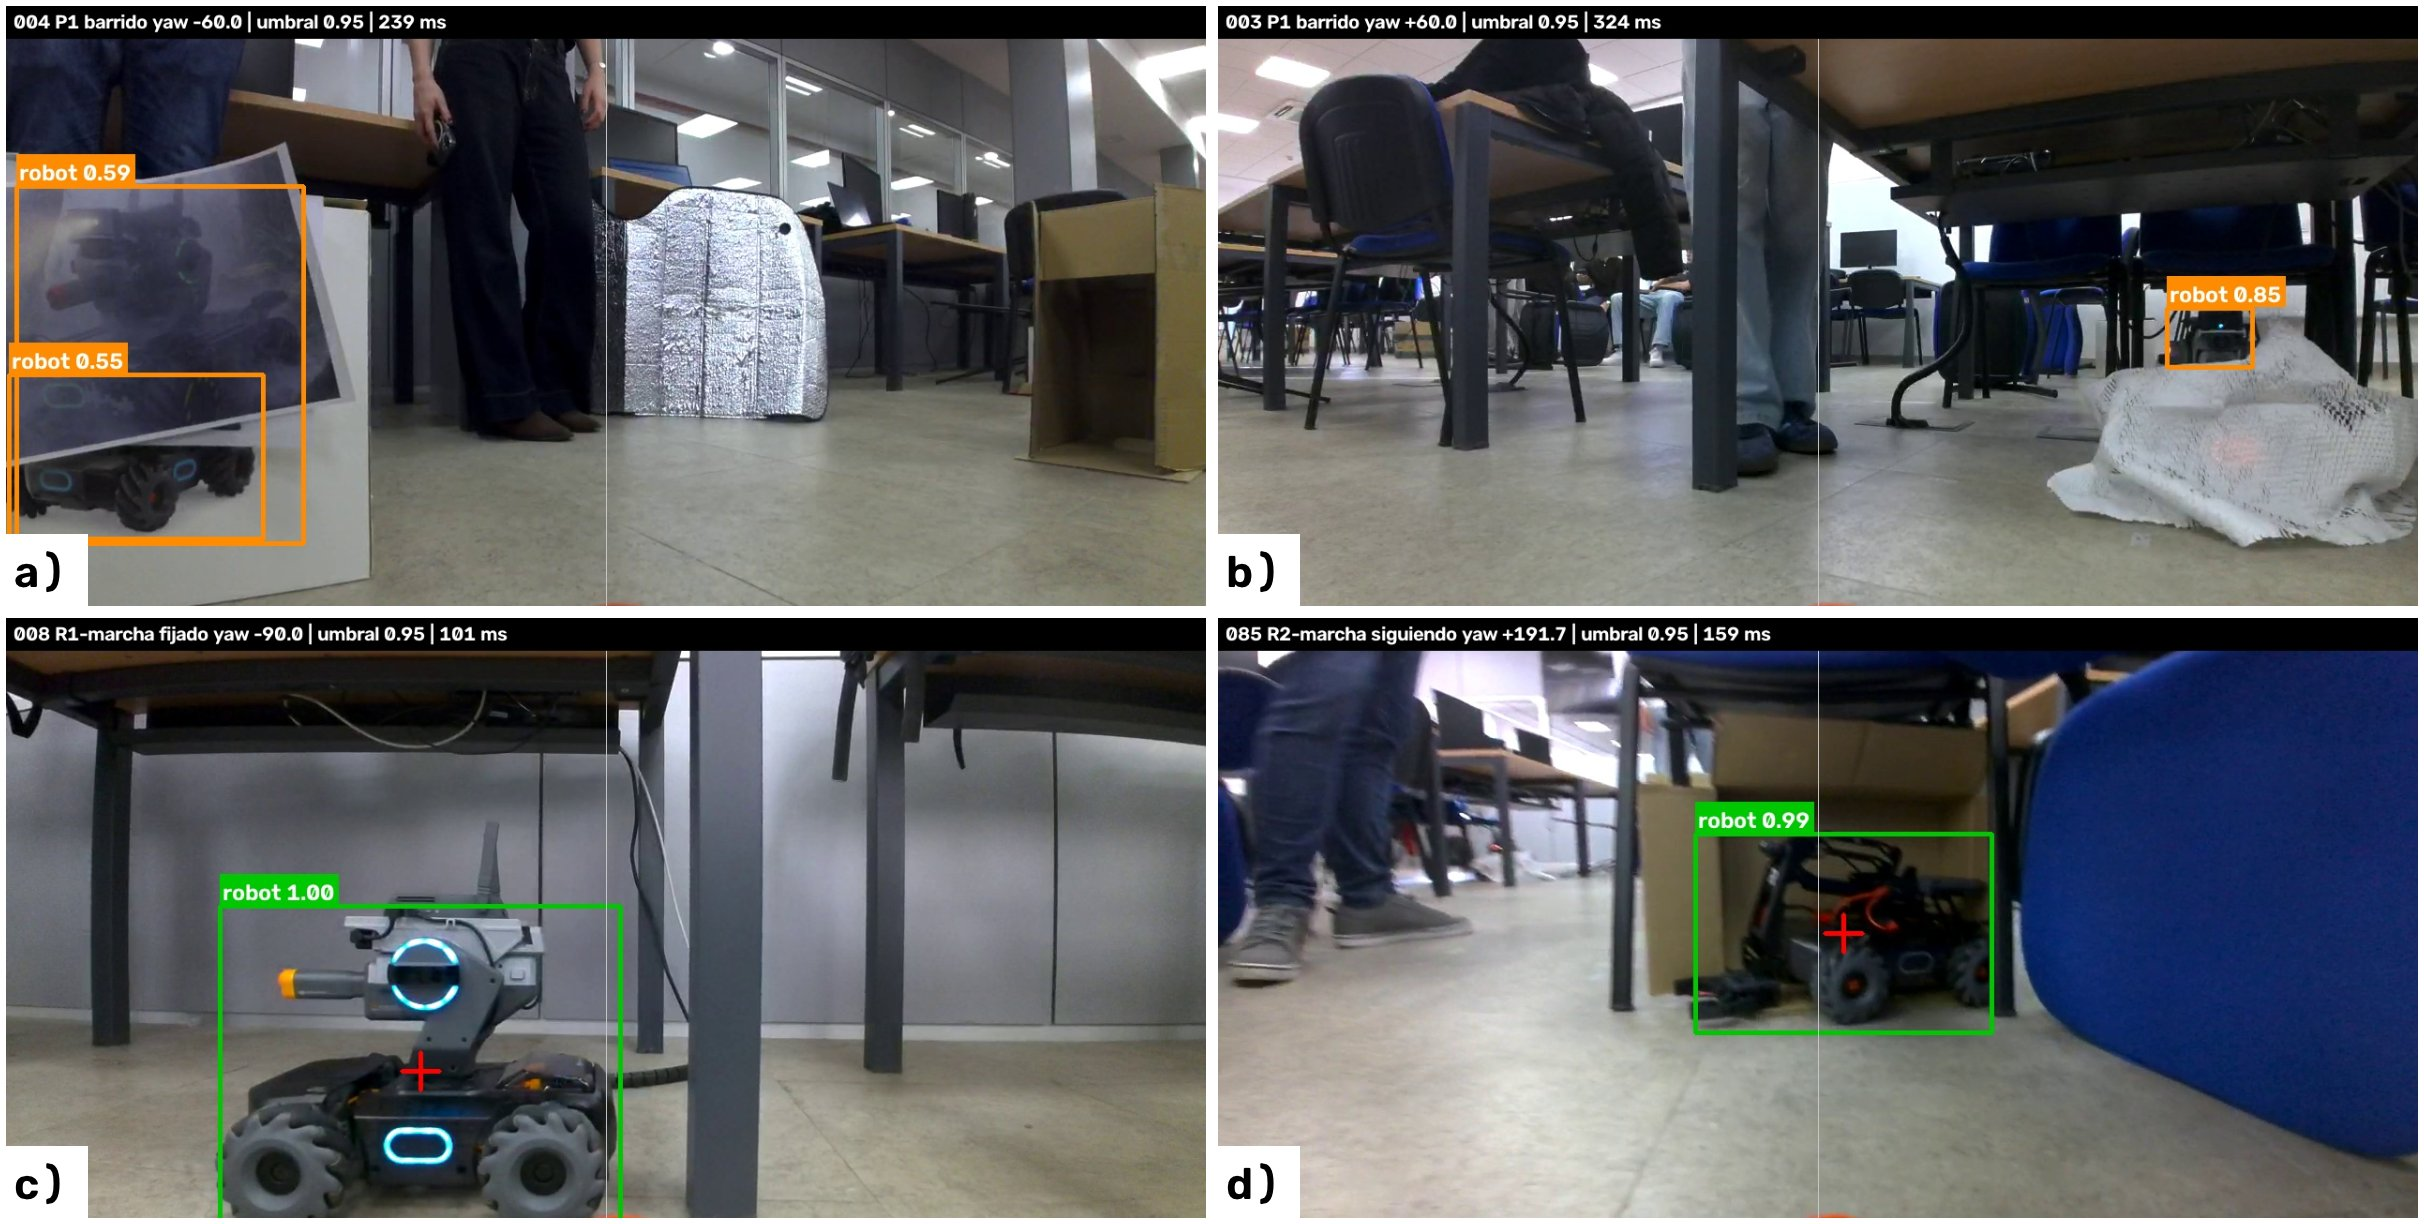
\includegraphics[width=0.85\textwidth]{intento_profesor.jpg}
\caption{Intento sorpresa del profesor.}
\end{figure}

\subsection{Seguridad (muy preguntable)}
\begin{itemize}
  \item Toda orden \cod{drive\_\allowbreak{}speed} caduca a los 0,5 s: si el programa se cuelga, el robot se para solo.
  \item \cod{cerrar()} en un \cod{finally}: con error o Ctrl+C se para el chasis, se centra la torreta y se apagan los LED.
  \item Batería: con menos del 10\,\% no arranca; con menos del 20\,\% avisa.
  \item Disparar solo a robots: umbral 0,95, filtro de cajas altas, distancia máxima en P1 y confirmación antes de la ráfaga.
  \item Velocidades máximas: 0,5 m/s y 30\gr/s. El rival móvil nunca pasa de 0,1 m/s y exige el número de serie del rival para no conectarse por error a nuestro robot.
\end{itemize}

\subsection{Mejoras implementadas pero desactivadas}
\cod{SEGUIMIENTO}, \cod{BARRIDO\_\allowbreak{}CONTINUO}, \cod{MEMORIA}, \cod{VIGILANCIA} y \cod{LEER\_\allowbreak{}ANGULO\_\allowbreak{}GIMBAL} están programadas y probadas en simulación pero \textbf{a \texttt{False}} porque no se validaron en el laboratorio: la demo hace lo probado y las mejoras se activan una a una, en ese orden. Es una decisión de ingeniería defendible (no incluir en la demo lo que no está comprobado) y conviene explicarla así.

\newpage
% =====================================================================
\section{La interfaz del mando}

Interfaz web para manejar el robot desde el portátil, con teclado y ratón o mando de PS4. Muestra el vídeo con las detecciones, mueve chasis y torreta, dispara y lanza bailes con los \emph{mismos topes de velocidad} que la demo. Probada con el robot real el 11/11: vídeo a 8--16 imágenes por segundo y detecciones con confianzas de 0,97 a 1,00, también con varios robots a la vez y detrás de obstáculos. Tiene 42 pruebas automáticas.

\begin{figure}[H]
\centering
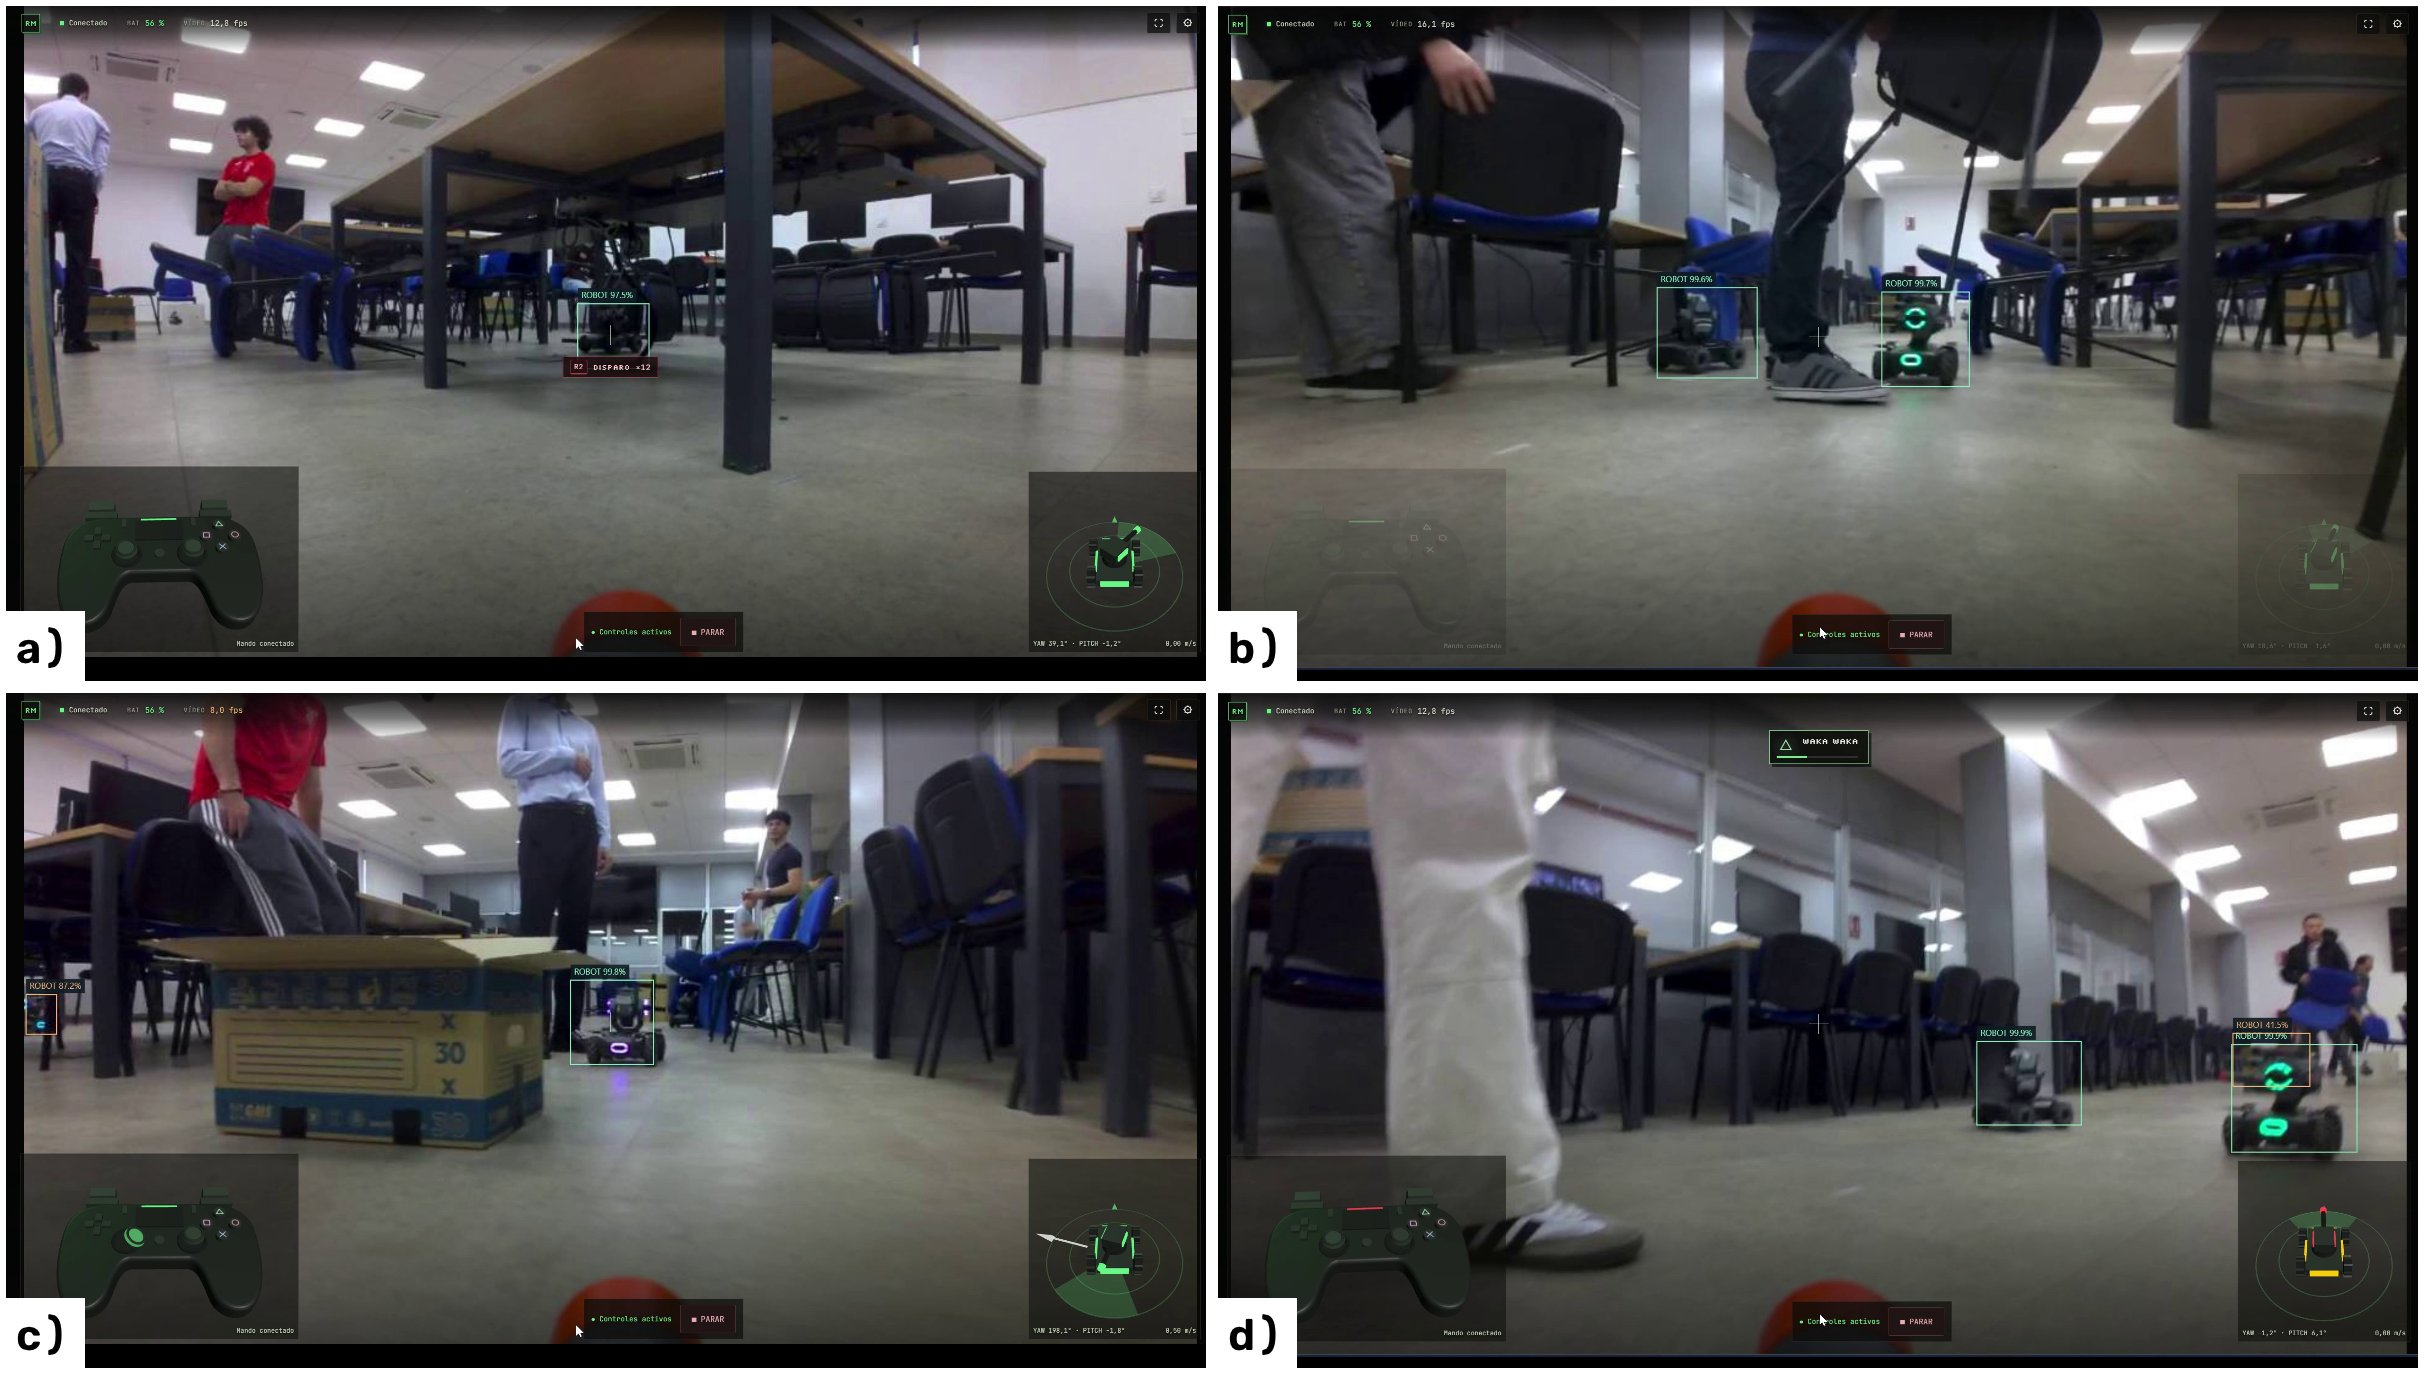
\includegraphics[width=0.8\textwidth]{interfaz_real.jpg}
\caption{Interfaz del mando con el robot real.}
\end{figure}

\textbf{Decisiones de diseño interesantes:}
\begin{itemize}
  \item \textbf{Un solo hilo habla con el SDK} (\cod{conductor.py}) para que dos órdenes no se pisen. El servidor y el detector solo dejan datos; el conductor decide. Bucle de control cada 25 ms.
  \item \textbf{Señal de vida:} el navegador manda el control cada 50 ms; si no llega nada en 0,3 s, el robot se para y se desarma (pestaña cerrada, wifi caído\ldots).
  \item \textbf{Una sola sesión de control:} la última pestaña que se conecta se queda el control y, al cambiar de propietario, el robot se para. El servidor solo escucha en \cod{127.0.0.1} y rechaza páginas de otro origen para que otra web no pueda mover el robot.
  \item \textbf{Vídeo MJPEG} sobre HTTP (\cod{multipart/\allowbreak{}x-mixed-replace}), reducido a 960$\times$540.
  \item \textbf{Disparo automático opcional:} solo si hay caja $\ge$0,95 bajo la mira, la detección tiene $<$0,5 s y la torreta no se ha movido más de 2\gr{} desde la foto. También hay asistente de puntería que centra la torreta en el rival.
  \item \textbf{Bailes como funciones del tiempo} (Moonwalk, Waka Waka, Super Estrella, Risa). Cada uno se \emph{simula} antes de usarse: se integra el movimiento y se comprueba que no pasa de 0,5 m/s ni 30\gr/s, cabe en 1$\times$1 m y \textbf{vuelve al punto de partida}.
  \item Los controles 3D con Three.js van copiados en local, porque en la wifi del robot no hay internet.
\end{itemize}

\textbf{El límite es el hardware.} El RoboMaster solo envía el vídeo por wifi y recibe órdenes, así que el detector va en el portátil. En la demo, unos 108 ms por imagen; con la interfaz, que además muestra el vídeo, el disparo automático del 12/11 tardó de 130 a 570 ms. Para que fuera fluido haría falta una GPU de sobremesa o un modelo más ligero, y para no depender de la wifi, un ordenador con GPU a bordo y un router propio.

% =====================================================================
\section{Material de apoyo para la presentación}
\begin{itemize}
  \item \textbf{Presentación} (\cod{presentacion/\allowbreak{}}): 26 diapositivas en React + Vite. Teclas en la sección~\ref{sec:guion}. Los datos de las gráficas salen del repositorio con \cod{npm run datos} (\cod{scripts/\allowbreak{}preparar\_\allowbreak{}datos.mjs}), que falla si las cifras del EDA no coinciden con las de la memoria.
  \item \textbf{Zip para Moodle:} la presentación en un solo fichero HTML (doble clic, sin conexión) y un PDF estático con una página por diapositiva.
  \item \textbf{Web en GitHub Pages} (\cod{web/\allowbreak{}}): figuras interactivas de los tres bloques; la del Bloque 3 muestra la demo foto a foto, qué vio el detector y cuánto duró cada fase.
  \item \textbf{Memoria}: incluye la tabla «Respuesta a la revisión anterior» (16 comentarios de la entrega 2, todos atendidos): esquema de bloques, SGD citado, una etapa frente a dos, batch size justificado, tasa baja, momentum y programador, curva PR, resoluciones, \emph{difficult} en validación y test, FPN, notación científica, puntos porcentuales\ldots
  \item \textbf{Documentos útiles del repositorio:} \cod{docs/\allowbreak{}revision\_\allowbreak{}fp\_\allowbreak{}test.csv} (los 94 FP), \cod{docs/\allowbreak{}senuelo\_\allowbreak{}aliado.md} (robot camuflado y aliados), \cod{docs/\allowbreak{}seleccion\_\allowbreak{}modelo\_\allowbreak{}final.md} (regla fijada antes del test), \cod{ENTREGA 2/\allowbreak{}WEEK3/\allowbreak{}README.md} (demo) y los notebooks del EDA y del aumento ejecutados en HTML.
\end{itemize}

\newpage
% =====================================================================
\section{Mapa de decisiones: qué salió bien, qué falló y por qué}\label{sec:mapa}

Los profesores insistieron en la \textbf{justificación}: no se valora tanto que algo funcione como saber \emph{por qué} funcionó o falló y qué se aprendió. Esta sección reúne las decisiones del proyecto con ese formato. Cada fila se puede contar en 20 segundos.

\subsection{Decisiones que salieron bien}
\begin{longtable}{@{}P{3.6cm}P{5.4cm}P{5.5cm}@{}}
\toprule
\textbf{Decisión} & \textbf{Por qué se tomó} & \textbf{Qué demostró} \\
\midrule
\endhead
Elegir el intervalo de extracción midiendo & Con 12 el doble de trabajo; con 48 la mitad de ejemplos & 808 imágenes con un 1,4\,\% de casi duplicadas \\
Entrenar con nuestros datos y evaluar con los de otros grupos & Los fotogramas de un vídeo se parecen entre sí (74\,\% de vecinos del mismo vídeo): mezclarlos inflaría el resultado & Test 0,9523 $\approx$ validación 0,9513: la medida es honesta, no hay fuga \\
Escribir la regla de selección antes de abrir el test & Evitar elegir modelo mirando el test & Nadie puede decir que el modelo se ajustó al test; empates $<$0,5 pp se resuelven por coste \\
Aumento propio en vez del del notebook & El del notebook recorta 640$\times$480, ensancha los robots un 33\,\% y pierde el 14,1\,\% de ellos; el nuestro, 0,7\,\% & +8 pp de AP en \emph{difficult} y 28\,\% menos de robots perdidos \\
Transformaciones elegidas por el EDA & Franja de altura, tamaño según posición, forma estable, robots movidos & Ninguna escena imposible; cajas que siguen ajustadas \\
Marcar \emph{difficult} (también en validación y test) y evaluarlos aparte & Un AP global alto esconde los casos duros & Se vio que el 64\,\% de los fallos son \emph{difficult} (el 16\,\% de los robots) \\
Revisar los FP uno a uno & Saber si el modelo falla o faltan etiquetas & Solo 4 de 94 no son robots; 59 son etiquetas que faltan \\
Umbral 0,95 fijado en validación & En la demo un falso disparo es peor que perder un objetivo & No disparó al robot tapado ni a la foto con humo del profesor \\
Detector en un proceso aparte con GPU & SDK atado a Python 3.8; PyTorch de 3.8 no soporta la RTX 5070 & De unos 2,3 s a unos 108 ms por imagen sin tocar el SDK, y con respaldo a CPU \\
Hilo que lee el vídeo y guarda solo la última imagen & La cola del SDK (64 imágenes) se llenaba con imágenes viejas & Se acabó el «detecta pero no dispara» \\
Usar el ángulo de la torreta \emph{del instante de la foto} & La imagen llega con retraso & La puntería deja de ir siempre por detrás del objetivo \\
Calcular velocidades sumando tiempos & Giro 3 s + ver + voz 1,4 s + ráfaga 6,2 s & El ataque en marcha al rival 2 cupo en el tramo (14,5 s a 0,1 m/s) \\
Medir el sentido de la corrección con la IMU & Se había supuesto el signo y estaba mal & Corrige hacia donde debe, no al revés \\
Mejoras desactivadas si no están validadas & Sin probar en laboratorio no se puede garantizar que no rompan la demo & La demo hace solo lo comprobado; se activan una a una \\
\bottomrule
\end{longtable}

\subsection{Lo que falló (o se descartó) y la lección}
\begin{longtable}{@{}P{3.3cm}P{5.2cm}P{6cm}@{}}
\toprule
\textbf{Qué pasó} & \textbf{Por qué} & \textbf{Lección / qué se hizo} \\
\midrule
\endhead
Rival 3 sin eliminar en la demo oficial & Fijó primero un robot del fondo y descartó al rival 3 por estar a más de 25\gr{} del fijado & La detección fue buena; falló a quién fijar. Aplicar el filtro de distancia también en marcha \\
Resolución 1024 px & AP pequeños sube de 0,12 a 0,19 pero con 134 FP más y +62\,\% de latencia (75 $\rightarrow$ 122 ms) & Una mejora no es uniforme: se mide en todas las métricas, no solo en la que sube. Se descartó \\
Extras del aumento (\cod{robusto\_\allowbreak{}v1}) & Mismo AP que el base (0,9426 frente a 0,9433) & No empeoran y cubren casos no grabados; validación casi sin exteriores no puede medir lo que aportan \\
SSD y SSDlite muy por debajo (AP 0,88 y 0,64) & Reducen la imagen a 300--320 px: los robots lejanos quedan minúsculos & Velocidad no compensa si se pierden los objetivos difíciles (AP \emph{difficult} 0,43 y 0,27) \\
Tasas $10^{-5}$, $10^{-1}$ y $2\cdot10^{-3}$ & $10^{-5}$ casi no aprende, $10^{-1}$ da NaN y $2\cdot10^{-3}$ alcanza el máximo en la época 1--2 y luego baja más de 1 pp & Entre $10^{-4}$ y $10^{-2}$ solo cambia la velocidad; se usó $10^{-3}$ \\
Programador con paciencia de 5 & El estancamiento ocurre en 2--3 épocas & Reconocido en la memoria: haría falta una prueba de rango de la tasa \\
30 épocas & En 6 de 7 modelos el mejor \emph{checkpoint} está entre las épocas 3 y 7 & No faltaban épocas: hay sobreajuste temprano. Se redujo a 12--15 y se guarda el mejor \emph{checkpoint} \\
Lotes de 1--2 imágenes & Suben antes pero bajan en la tercera época & Con lote 8 la subida es más regular; es el mayor que cabe en 12 GB \\
Perspectiva y giros de 90\gr{} en el aumento & Con Albumentations 1.4.18 la perspectiva desplaza mal las cajas (prueba automática); los giros de 90\gr{} ponen el robot de lado & Se probó cada transformación antes de usarla; se descartaron \\
Etiquetas de otros grupos incompletas & 59 de los 94 FP de test son robots sin anotar & No se corrigieron para conservar la comparación; se declara y se cuantifica \\
Borde superior de las cajas & Los cinco discrepamos (mediana de 7 px frente a 4--5 px) por gimbal y antenas & IoU entre anotadores 0,81, no mayor. Cerrar el criterio queda pendiente (T01) \\
Robots «aliados» (señuelo) & El detector los reconoce a todos como robot (92,7--99,9\,\%); tapando partes apenas baja & El modelo aprendió el concepto, no una pieza. Idea reconvertida: robot camuflado = objetivo más; aliados con marca de color, como trabajo futuro \\
Robot sin disparar pese a detectarlo (0,96--1,00) & Imágenes con franjas o antiguas por la cola de vídeo & Primer gran bug de integración; se resolvió con el hilo de última imagen \\
Avance a 0,06 m/s y desvío al ir recto & \cod{chassis.move} no da m/s reales; las ruedas decían «recto» pero el chasis giraba & \cod{drive\_\allowbreak{}speed} más bucle odometría + IMU \\
Sillas y robots del fondo como robot & Cajas enormes (robot a $<$0,5 m) o lejanas & Filtro de caja alta y distancia máxima en P1 \\
Tramos del recorrido del plano & Las pruebas de laboratorio obligaron a corregir tramos (+15\,\% tras el túnel) & Medir en el laboratorio, no confiar en el plano \\
Robot tapado (0,85--0,91) y foto con humo (0,59) sin disparo & Quedan bajo el umbral 0,95 & Es el \emph{coste} de un umbral alto: se asume y se explica \\
\bottomrule
\end{longtable}

\begin{clave}
Patrón que se repite y que conviene verbalizar: \textbf{casi todos los fallos vinieron de suponer algo en lugar de medirlo o comprobarlo} (el signo de la IMU, los metros del plano, la cola de vídeo, la resolución como mejora, que el primer robot visto en R2 sería el rival 3). Las decisiones que funcionaron se tomaron con una medida o una regla fijada antes.
\end{clave}

\newpage
% =====================================================================
\section{Preguntas probables y cómo responderlas}\label{sec:preguntas}

\subsection*{Datos}

\begin{pregunta}{¿Por qué dos conjuntos distintos para entrenar y evaluar?}
Entrenamos con nuestros 10 vídeos y validamos/testeamos con los conjuntos de otros grupos de la asignatura. Así no hay fuga entre conjuntos (los fotogramas de un mismo vídeo se parecen mucho: el vecino más parecido es del mismo vídeo en el 74\,\% de los casos) y medimos en escenas que el modelo no ha visto. Coste: no controlamos sus etiquetas (59 de los 94 FP de test son robots que faltan en sus XML).
\end{pregunta}

\begin{pregunta}{¿No sesgáis el resultado al marcar vosotros los \emph{difficult} de validación y test?}
No cambia el AP global: solo se añadió la marca, sin tocar ninguna caja. Sirve para medir aparte los casos difíciles con nuestro criterio: 48 robots de menos de 30 px directamente y 477 de 930 candidatos revisados a ojo, recortados y ampliados.
\end{pregunta}

\begin{pregunta}{¿Para qué sirvió el EDA?}
Cada análisis dio una decisión (tabla de la sección~\ref{sec:bloque1}): la franja de altura limita el desplazamiento vertical; la relación tamaño--posición impide deformar; la forma estable deja las anclas por defecto; el solapamiento máximo de 0,26 valida la NMS a 0,5; la nitidez justifica el desenfoque de movimiento; y la comparación con validación anticipó los dos puntos débiles del modelo (\emph{difficult} y robots lejanos).
\end{pregunta}

\begin{pregunta}{¿Por qué no anotar las antenas?}
Solo se ven de cerca. Con ellas, el borde superior de la caja dependería de la distancia, y la caja cambiaría de tamaño y de centro de forma inconsistente. Aun así, el borde superior es donde más discrepamos los cinco (7 px de mediana).
\end{pregunta}

\subsection*{Modelo}

\begin{pregunta}{¿Qué aportó más, el aumento o la arquitectura?}
Son preguntas distintas. Frente a no aumentar, el aumento fue la mejora más importante, sobre todo en \emph{difficult} (+8 pp y 28\,\% menos de robots perdidos). Entre modelos ya entrenados con aumento, la arquitectura influye más que la tasa o el perfil de aumento: la tasa mueve menos de 0,22 pp y el perfil, 0,07 pp.
\end{pregunta}

\begin{pregunta}{¿Por qué AP@0,5 alto pero AP 0,50:0,95 bajo?}
El modelo encuentra los robots pero muchas cajas tienen IoU $<$0,75 (AP@0,75 = 0,60). En parte es por las etiquetas de otros grupos (criterio distinto con antenas y robots cortados): ni siquiera nosotros coincidíamos en el borde superior. Para disparar basta con encontrar el robot y apuntar al centro.
\end{pregunta}

\begin{pregunta}{¿Cómo sabéis que no habéis sobreajustado al test?}
La regla de selección se escribió antes de abrir el test y cada modelo se evaluó una única vez, con el umbral ya fijado en validación. El test no se usó para elegir nada. Y validación y test dan casi lo mismo (0,9513 y 0,9523).
\end{pregunta}

\begin{pregunta}{¿Por qué no habéis probado YOLO u otros detectores?}
Respuesta honesta: no lo comparamos. Nos centramos en los detectores de torchvision, que comparten código de entrenamiento y evaluación, para que la comparación fuera justa. Con lo medido, el cuello de botella no era la arquitectura sino los \emph{difficult} y las etiquetas; un detector más rápido sería una mejora para la interfaz, no para la demo.
\end{pregunta}

\begin{pregunta}{¿Por qué la exactitud no aparece en las conclusiones?}
Porque en detección no hay verdaderos negativos: el fondo no es un objeto y el test no tiene imágenes vacías. Con TN = 0 la exactitud es TP/(TP+FP+FN) (0,8848) y no aporta nada que no den precisión y exhaustividad.
\end{pregunta}

\subsection*{Robot}

\begin{pregunta}{¿Por qué no se eliminó al rival 3?}
Lo detectó con 1,00, pero antes había fijado un robot del fondo (0,99) y giró hacia él. El rival 3 apareció a 30--36\gr{} de la línea de tiro, más de los 25\gr{} con los que el seguimiento decide que es «otro robot», así que lo ignoró en 43 imágenes y los disparos le pasaron por la izquierda. El filtro de distancia de P1, aplicado también en marcha, habría descartado el robot del fondo (sección~\ref{sec:rival3}).
\end{pregunta}

\begin{pregunta}{¿La demo es robusta o funcionó una vez?}
Hubo pruebas de laboratorio del 4 al 11/11 que corrigieron la cola de vídeo, los tramos del recorrido (+15\,\% tras el túnel), las sillas y los robots del fondo. En la demo oficial eliminó a 3 de 4 y el fallo está explicado; el intento sorpresa del profesor mostró los límites (robot tapado y foto con humo no alcanzan 0,95). Es una demo \emph{con límites conocidos y explicados}.
\end{pregunta}

\begin{pregunta}{¿Por qué no usasteis la GPU desde el principio?}
Porque el SDK exige Python 3.8, cuyo PyTorch no admite la RTX 5070. La solución fue un proceso aparte con Python 3.11 y CUDA 12.8 y comunicación local, con respaldo a CPU.
\end{pregunta}

\begin{pregunta}{¿Cómo calculáis cuánto girar la torreta?}
Con la distancia en píxeles entre el centro de la caja y el centro de la imagen y la distancia focal equivalente: $\alpha = \arctan(\text{desvío}/f)$, corregido por el campo de visión medido ($\approx$90\gr). Se usa el ángulo de la torreta en el instante de la foto, no el actual, y se confirma con otra imagen antes de disparar.
\end{pregunta}

\begin{pregunta}{¿Qué pasa si se cae la wifi o se cuelga el programa?}
Las órdenes de movimiento caducan a los 0,5 s, así que el robot se para solo. En la interfaz, si no llega nada en 0,3 s, se para y se desarma. Con un error o Ctrl+C, \cod{cerrar()} para el chasis, centra la torreta y apaga los LED.
\end{pregunta}

\begin{pregunta}{¿Por qué falló la idea de los aliados?}
Porque el detector aprendió el concepto de robot, no una pieza concreta: reconoce incluso robots disfrazados o generados con IA (92,7--99,9\,\%). Distinguirlos exige una señal distinta de la forma, como una marca de color (5,7--12,5\,\% de verde frente a 0\,\%); no se implementó por riesgo de falsos positivos con la luz del laboratorio.
\end{pregunta}

\subsection*{Generales}

\begin{pregunta}{¿Qué haríais con más tiempo?}
(1) Aplicar el filtro de distancia también en los ataques en marcha (el fallo del rival 3); (2) mejorar los \emph{difficult} (0,69 en test) con datos reales de robots tapados y lejanos; (3) varias semillas para cerrar diferencias $<$0,5 pp; (4) distinguir aliados con una marca de color; (5) activar y validar el seguimiento continuo y la vigilancia del recorrido; (6) grabar el circuito real y escenas con poca luz para el entrenamiento; (7) un ordenador con GPU a bordo para no depender de la wifi.
\end{pregunta}

\begin{pregunta}{¿Qué fue lo que peor salió y qué aprendisteis?}
Lo más costoso fue la integración, no la red: la cola de vídeo que daba imágenes viejas (el robot detectaba y no disparaba), el retraso de la cámara, la GPU incompatible con el SDK y, en la demo, fijar el robot equivocado. Aprendimos que hay que \emph{medir} en lugar de suponer, y que separar procesos y tener un respaldo (CPU) convierte un problema bloqueante en uno controlado.
\end{pregunta}

\begin{pregunta}{¿Qué hizo cada uno?}
Ver el reparto de la sección~\ref{sec:reparto}. Cada uno debe poder contar su parte y la de al menos otro bloque.
\end{pregunta}

\newpage
% =====================================================================
\section{Reparto del trabajo}\label{sec:reparto}
Resumen de la Tabla 1 de la memoria. Conviene que cada uno se sepa su fila: es habitual que pregunten a alguien por lo que hizo.

{\small
\begin{longtable}{@{}P{2.3cm}P{4.2cm}P{3.8cm}P{4.2cm}@{}}
\toprule
\textbf{Integrante} & \textbf{Bloque 1} & \textbf{Bloque 2} & \textbf{Bloque 3} \\
\midrule
\endhead
Javier Saguar & Lote A (vídeos 01--02); fichas de los vídeos, criterios de anotación y depuración; aumento sobre el script de Alejandro; redacción & Cadena de entrenamientos, evaluación final en test, comprobación con 40 épocas; gráficas de la web y la memoria & Demo del circuito (desplazamientos, puntería, disparo, ataques en marcha, camuflado), demo en GPU, kit del rival móvil, interfaz del mando y memoria del Bloque 3 \\
Alejandro Cuevas & Lote B (03--04); EDA y script de entrenamiento sobre el que se integró el aumento; redacción & Adaptación del código de entrenamiento y test, propuestas de mejora y memoria del Bloque 2 & Seguimiento de rivales en movimiento, barrido continuo, memoria de robots atacados y vigilancia del recorrido \\
Mónica Fernández & Lote C (05--06); calibración entre anotadores y revisión de la memoria & Correcciones de la memoria del Bloque 1 & Diseño del boceto del circuito \\
Pedro José Orrego & Lote D (07--08); calibración, figuras del EDA y web de figuras interactivas & Web interactiva del Bloque 2 y navegación común & Conexión y preparación del boceto de la demo \\
Daniel Naval & Lote E (09--10); calibración y redacción & -- & Ayuda en el montaje del circuito \\
\bottomrule
\end{longtable}
}

% =====================================================================
\section{Cifras para tener en la cabeza}\label{sec:cifras}

\begin{center}
\small
\begin{tabular}{@{}P{8.2cm}P{6.2cm}@{}}
\toprule
\multicolumn{2}{@{}l}{\textbf{Datos}} \\
Vídeos / duración / fotogramas & 10 / 643,8 s / 19\,508 \\
Intervalo / imágenes extraídas / tras depurar & 24 fotogramas / 808 / 796 \\
Robots / \emph{difficult} (originales) & 1420 / 375 (26,4\,\%) \\
IoU medio entre anotadores & 0,81 (borde superior: 7 px) \\
Franja de los centros / aspecto mediano & 0,37--0,58 del alto / 1,11 \\
Parejas que se tocan / IoU máximo & 92 de 809 / 0,26 \\
\emph{Difficult} en el cuarto menos / más nítido & 55\,\% / 11\,\% \\
Entrenamiento tras aumento & 3184 imágenes, 5566 cajas \\
Validación / test (asignatura) & 672 / 718 imágenes; 255 / 270 \emph{difficult} \\
\midrule
\multicolumn{2}{@{}l}{\textbf{Modelo}} \\
Entrenamientos en la cadena / horas de GPU & 13 / 21,8 h \\
Efecto del aumento (Faster R-CNN v1, validación) & 0,923 $\rightarrow$ 0,942; \emph{difficult} +8 pp \\
Perfil \cod{robusto\_\allowbreak{}v1} frente al base & 0,9426 frente a 0,9433 \\
Modelo final & Faster R-CNN v2, lr $10^{-3}$, época 3 \\
AP@0,5 validación / test & 0,9513 / 0,9523 \\
AP@0,5 test normales / \emph{difficult} & 0,9658 / 0,6921 \\
AP@0,75 / AP 0,50:0,95 en test & 0,6005 / 0,5724 \\
Umbral / TP / FP / FN en test & 0,95 / 1606 / 94 / 115 \\
Precisión / exhaustividad / F1 & 0,9447 / 0,9332 / 0,9389 \\
FP: sin anotar / mal ajustados / no robots & 59 / 31 / 4 (precisión corregida 0,979) \\
FN que son \emph{difficult} & 74 de 115 (64\,\%) \\
Latencia modelo final / MobileNet (RTX 3060) & 99,5 ms / 16 ms \\
\midrule
\multicolumn{2}{@{}l}{\textbf{Robot}} \\
Latencia en el robot: CPU / GPU & $\approx$2,3 s / $\approx$108 ms por imagen \\
Latencia con la interfaz & 130--570 ms por imagen \\
Disparos por robot / exigidos & 20 / 12 (uno cada 0,3 s, 6,2 s) \\
Velocidades máximas & 0,5 m/s y 30\gr/s; 0,1 m/s atacando \\
Umbral general / hacia el camuflado & 0,95 / 0,7 \\
\texttt{SALTO\_MAX} / distancia máxima en P1 & 25\gr{} / 2 m \\
Demo oficial (12/11) & 4 detectados, 3 eliminados (60 disparos) \\
Duración de la demo & $\approx$2 min 18 s \\
\midrule
\multicolumn{2}{@{}l}{\textbf{Entrega}} \\
Memoria & 46 páginas, cuerpo 4--32 (29) \\
Presentación & 26 diapositivas \\
\bottomrule
\end{tabular}
\end{center}

\end{document}
